\documentclass{article}
\usepackage{fancyhdr} % Required for custom headers
\usepackage{lastpage} % Required to determine the last page for the footer
\usepackage{extramarks} % Required for headers and footers
\usepackage[usenames,dvipsnames]{color} % Required for custom colors
\usepackage{graphicx} % Required to insert images
\usepackage{listings} % Required for insertion of code
\usepackage{courier} % Required for the courier font
\usepackage{lipsum} % Used for inserting dummy 'Lorem ipsum' text into the template
\usepackage{caption}
\usepackage{subcaption}
\usepackage{amsmath}
\usepackage{amsfonts}
\usepackage{amssymb}
\usepackage{epstopdf}
\usepackage{placeins}
\usepackage{color} 
\usepackage{fancyvrb} 
\usepackage{setspace}
\usepackage{array}
\usepackage[numbered]{bookmark}
\usepackage{tikz}
\usepackage{pgfplots}
\usepackage[absolute,overlay]{textpos}
\usetikzlibrary{calc, angles,quotes}
\usetikzlibrary{pgfplots.fillbetween, backgrounds}
\usetikzlibrary{positioning}
\usetikzlibrary{arrows}
\usetikzlibrary{pgfplots.groupplots}
\usetikzlibrary{arrows.meta}
\usetikzlibrary{plotmarks}
\usetikzlibrary{decorations.markings}

\usepgfplotslibrary{groupplots}
\pgfplotsset{compat=newest} 
%\pgfplotsset{plot coordinates/math parser=false}
\DeclareGraphicsExtensions{.pdf,.png,.jpg}
\graphicspath{{figs/}}

\definecolor{matlabcomment}{RGB}{34,139,34}

\pgfmathdeclarefunction{gauss}{1}{%
	\pgfmathparse{1/(sqrt(2*pi))*exp(-((#1)^2)/2)}%
}

\pgfmathdeclarefunction{laplacian}{2}{%
	\pgfmathparse{1/(#2*2)*exp(-(abs(x-#1))/(#2))}%
}

\pgfmathdeclarefunction{pretty_func}{1}{%
	\pgfmathparse{cos(deg(#1/2)) - sin(deg(#1)) + cos(deg(#1/2)-45) - sin(deg(#1/4)-154)}%
}

\pgfplotsset{
	dirac/.style={
		mark=triangle*,
		mark options={scale=2},
		ycomb,
		scatter,
		visualization depends on={y/abs(y)-1 \as \sign},
		scatter/@pre marker code/.code={\scope[rotate=90*\sign,yshift=-2pt]}
	}
}

\def\thickness{very thick}

\tikzset{
amark/.style 2 args={
	decoration={             
		markings, 
		mark=at position {0.5} with { 
			\arrow{stealth},
			\node[#2] {#1};
		}
	}, \thickness,
	postaction={decorate}
},
earlymark/.style 2 args={
	decoration={             
		markings, 
		mark=at position {0.25} with { 
			\arrow{stealth},
			\node[#2] {#1};
		}
	}, \thickness,
	postaction={decorate}
},
latemark/.style 2 args={
	decoration={             
		markings, 
		mark=at position {0.8} with { 
			\arrow{stealth},
			\node[#2] {#1};
		}
	}, \thickness,
	postaction={decorate}
},
zpath/.style={
	decoration={             
		markings, 
		mark=at position {0.5} with { 
			\arrow{stealth},
			\node[#1] {$z^{-1}$};
		}
	}, \thickness,
	postaction={decorate}
},
terminal/.style 2 args={draw,circle,inner sep=2pt,label={#1:#2}},
}


\tikzset{
	invisible/.style={opacity=0},
	visible on/.style={alt={#1{}{invisible}}},
	alt/.code args={<#1>#2#3}{%
		\alt<#1>{\pgfkeysalso{#2}}{\pgfkeysalso{#3}} % \pgfkeysalso doesn't change the path
	},
}

\newcommand\PlotSampledSpectrum[4]{%
	\def\fs{#2}%
	\def\fmax{#3}%
	\def\ros{#4}%
	\input{#1}%
}

\pgfmathdeclarefunction{invgauss}{2}{%
	\pgfmathparse{sqrt(-2*ln(#1))*cos(deg(2*pi*#2))}%
}

\tikzset{
	declare function={
		sinc(\x) = (and(\x!=0, 1) * (sin(deg(pi*\x))/(pi*\x)) +
		(and(\x==0, 1) * 1);
	}
}

%\DeclareMathOperator{\E}{\mathbb{E}} % expectation

\newcommand\SimpleSys[4]{%
	\def\xin{#2}%
	\def\Hz{#3}%
	\def\yout{#4}
	\input{#1}%
}

% Margins
\topmargin=-0.45in
\evensidemargin=0in
\oddsidemargin=0in
\textwidth=6.5in
\textheight=9.0in
\headsep=0.25in

\linespread{1.2} % Line spacing

% Set up the header and footer
\pagestyle{fancy}
\lhead{\hmwkAuthorName} % Top left header
\chead{\hmwkTitle} % Top center head
\rhead{\hmwkClass} % Top right header
\lfoot{} % Bottom left footer
\cfoot{} % Bottom center footer
\rfoot{Page\ \thepage\ of\ \protect\pageref{LastPage}} % Bottom right footer
\renewcommand\headrulewidth{0.4pt} % Size of the header rule
\renewcommand\footrulewidth{0.4pt} % Size of the footer rule

%\setlength\parindent{0pt} % Removes all indentation from paragraphs
\definecolor{MyDarkGreen}{rgb}{0.0,0.4,0.0} % This is the color used for comments
\lstloadlanguages{Perl} % Load Perl syntax for listings, for a list of other languages supported see: ftp://ftp.tex.ac.uk/tex-archive/macros/latex/contrib/listings/listings.pdf
\lstset{language=Perl, % Use Perl in this example
        frame=single, % Single frame around code
        basicstyle=\small\ttfamily, % Use small true type font
        keywordstyle=[1]\color{Blue}\bf, % Perl functions bold and blue
        keywordstyle=[2]\color{Purple}, % Perl function arguments purple
        keywordstyle=[3]\color{Blue}\underbar, % Custom functions underlined and blue
        identifierstyle=, % Nothing special about identifiers                                         
        commentstyle=\usefont{T1}{pcr}{m}{sl}\color{MyDarkGreen}\small, % Comments small dark green courier font
        stringstyle=\color{Purple}, % Strings are purple
        showstringspaces=false, % Don't put marks in string spaces
        tabsize=5, % 5 spaces per tab
        %
        % Put standard Perl functions not included in the default language here
        morekeywords={rand},
        %
        % Put Perl function parameters here
        morekeywords=[2]{on, off, interp},
        %
        % Put user defined functions here
        morekeywords=[3]{test},
       	%
        morecomment=[l][\color{Blue}]{...}, % Line continuation (...) like blue comment
        numbers=left, % Line numbers on left
        firstnumber=1, % Line numbers start with line 1
        numberstyle=\tiny\color{Blue}, % Line numbers are blue and small
        stepnumber=5 % Line numbers go in steps of 5
}

% Creates a new command to include a perl script, the first parameter is the filename of the script (without .pl), the second parameter is the caption
\newcommand{\perlscript}[2]{
\begin{itemize}
\item[]\lstinputlisting[caption=#2,label=#1]{#1.pl}
\end{itemize}
}

% Header and footer for when a page split occurs within a problem environment
\newcommand{\enterProblemHeader}[1]{
\nobreak\extramarks{#1}{#1 continued on next page\ldots}\nobreak
\nobreak\extramarks{#1 (continued)}{#1 continued on next page\ldots}\nobreak
}

% Header and footer for when a page split occurs between problem environments
\newcommand{\exitProblemHeader}[1]{
\nobreak\extramarks{#1 (continued)}{#1 continued on next page\ldots}\nobreak
\nobreak\extramarks{#1}{}\nobreak
}

\setcounter{secnumdepth}{0} % Removes default section numbers
\newcounter{homeworkProblemCounter} % Creates a counter to keep track of the number of problems

\newcommand{\homeworkProblemName}{}
\newenvironment{homeworkProblem}[1][Problem \arabic{homeworkProblemCounter}]{ % Makes a new environment called homeworkProblem which takes 1 argument (custom name) but the default is "Problem #"
\stepcounter{homeworkProblemCounter} % Increase counter for number of problems
\renewcommand{\homeworkProblemName}{#1} % Assign \homeworkProblemName the name of the problem
\section{\homeworkProblemName} % Make a section in the document with the custom problem count
\enterProblemHeader{\homeworkProblemName} % Header and footer within the environment
}{
\exitProblemHeader{\homeworkProblemName} % Header and footer after the environment
}

\newcommand{\problemAnswer}[1]{ % Defines the problem answer command with the content as the only argument
\noindent\framebox[\columnwidth][c]{\begin{minipage}{0.98\columnwidth}#1\end{minipage}} % Makes the box around the problem answer and puts the content inside
}

\newcommand{\homeworkSectionName}{}
\newenvironment{homeworkSection}[1]{ % New environment for sections within homework problems, takes 1 argument - the name of the section
\renewcommand{\homeworkSectionName}{#1} % Assign \homeworkSectionName to the name of the section from the environment argument
\subsection{\homeworkSectionName} % Make a subsection with the custom name of the subsection
\enterProblemHeader{\homeworkProblemName\ [\homeworkSectionName]} % Header and footer within the environment
}{
\enterProblemHeader{\homeworkProblemName} % Header and footer after the environment
}

%----------------------------------------------------------------------------------------
%	NAME AND CLASS SECTION
%----------------------------------------------------------------------------------------
%%%%%%%%%%%%%%%%%%%%%%%%%%%%%%%%%%%%%%%%%%%%%%%%%%%%%%%%%%%%%%%%%%%%%%%%%%%%%%%%%%%%%%%%%
\newcommand{\hmwkTitle}{Homework \#05} % Assignment title
\newcommand{\hmwkDueDate}{\today} % Due date
\newcommand{\hmwkClass}{EE 264 (Summer 2018)} % Course/class
\newcommand{\hmwkAuthorName}{Solutions} % Your name
%%%%%%%%%%%%%%%%%%%%%%%%%%%%%%%%%%%%%%%%%%%%%%%%%%%%%%%%%%%%%%%%%%%%%%%%%%%%%%%%%%%%%%%%%
%----------------------------------------------------------------------------------------
%	TITLE PAGE
%----------------------------------------------------------------------------------------
\title{
\vspace{2in}
\textmd{\textbf{\hmwkClass:\ \hmwkTitle}}\\
\normalsize\vspace{0.1in}\small{Due\ on\ \hmwkDueDate}\\
\vspace{0.1in}\large{\textit{\hmwkClassInstructor\ \hmwkClassTime}}
\vspace{3in}
}

\author{\textbf{\hmwkAuthorName}}
\date{} % Insert date here if you want it to appear below your name

%----------------------------------------------------------------------------------------

\begin{document}
	
	
\section{Problem 1}

\subsection{(a)}

\begin{align} \nonumber
H(z) &= 0.05634\frac{(1+z^{-1})(1 -1.0166z^{-1} + z^{-2})}{(1-0.683z^{-1})(1 -1.4461z^{-1} + 0.7957z^{-2})} \\
&= 0.05634\frac{1+z^{-1}}{1-0.683z^{-1}}\cdot\frac{1 -1.0166z^{-1} + z^{-2}}{1 -1.4461z^{-1} + 0.7957z^{-2}}
\end{align}

To implement each subsystem you could choose whatever form. The picture below shows the implementation assuming a direct form II.

\begin{figure}[!h]
	\resizebox{0.9\textwidth}{!}{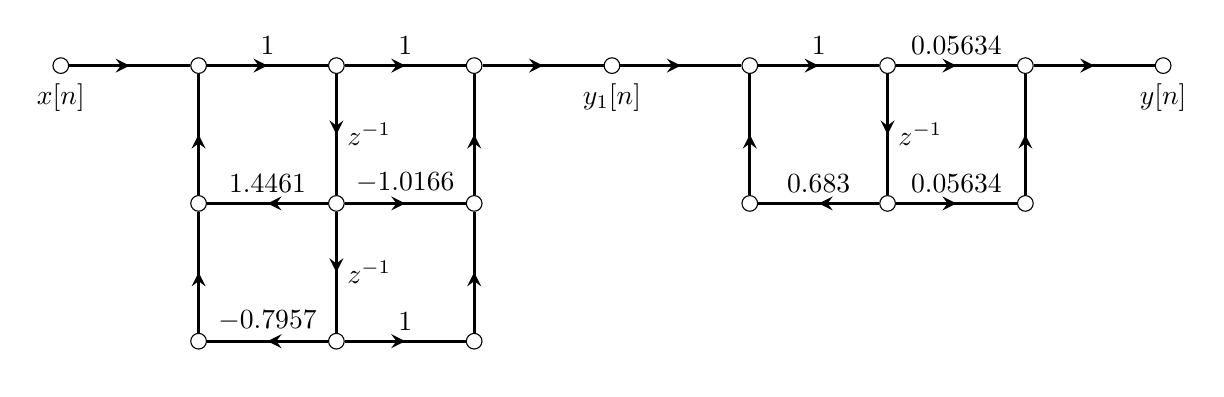
\begin{tikzpicture}[node distance=1.75cm]
%Place the nodes
\node[terminal={below}{$x[n]$}] (x) at (0,0) {};
\node[terminal={below}{}, right of=x] (00) {};
\node[terminal={below}{}, right of= 00] (01) {};
\node[terminal={below}{}, right of=01] (02) {};
\node[terminal={below}{$y_1[n]$}, right of=02] (y1) {};

\foreach \j in {1, 2} {
	\pgfmathtruncatemacro{\jn}{(\j-1)}%
	\node[terminal={below}{}, below of=\jn0] (\j0) {};
	\node[terminal={below}{}, below of=\jn1] (\j1) {};
	\node[terminal={below}{}, below of=\jn2] (\j2) {};
}

%
\draw[zpath={right}] (01) to (11);
\draw[zpath={right}] (11) to (21);

%
\draw[amark] (10) to (00);
\draw[amark] (20) to (10);

%
\draw[amark] (12) to (02);
\draw[amark] (22) to (12);

%
\draw[amark={$1$}{above}] (00) to (01);
\draw[amark={$1.4461$}{above}] (11) to (10);
\draw[amark={$-0.7957$}{above}] (21) to (20);

%
\draw[amark={$1$}{above}] (01) to (02);
\draw[amark={$-1.0166$}{above}] (11) to (12);
\draw[amark={$1$}{above}] (21) to (22);

\draw[amark] (x) to (00);
\draw[amark] (02) to (y1);


%Place the nodes
\node[terminal={below}{}, right of=y1] (00) {};
\node[terminal={below}{}, right of= 00] (01) {};
\node[terminal={below}{}, right of=01] (02) {};
\node[terminal={below}{$y[n]$}, right of=02] (y) {};

\foreach \j in {1} {
	\pgfmathtruncatemacro{\jn}{(\j-1)}%
	\node[terminal={below}{}, below of=\jn0] (\j0) {};
	\node[terminal={below}{}, below of=\jn1] (\j1) {};
	\node[terminal={below}{}, below of=\jn2] (\j2) {};
}

%
\draw[zpath={right}] (01) to (11);

%
\draw[amark] (10) to (00);

%
\draw[amark] (12) to (02);

%
\draw[amark={$1$}{above}] (00) to (01);
\draw[amark={$0.683$}{above}] (11) to (10);

%
\draw[amark={$0.05634$}{above}] (01) to (02);
\draw[amark={$0.05634$}{above}] (11) to (12);

\draw[amark] (y1) to (00);
\draw[amark] (02) to (y);

\end{tikzpicture}}
\end{figure}
\noindent\textbf{Notation warning:} the coefficients corresponding to the poles appear with a different sign, since the diagram assumes a transfer function of the form:

\begin{equation}
	H(z) = \frac{\sum_{k=0}^M b_kz^{-k}}{1-\sum_{k=1}^N a_kz^{-k}}
\end{equation}

\subsection{(b)}

\begin{align} \nonumber
H(z) &= 0.05634\frac{(1+z^{-1})(1 -1.0166z^{-1} + z^{-2})}{(1-0.683z^{-1})(1 -1.4461z^{-1} + 0.7957z^{-2})} \\
&= \frac{0.0563 -0.0009z^{-1}   -0.0009z^{-2}   + 0.0563z^{-3}}{1.0000   -2.1291z^{-1}    +1.7834z^{-2}   -0.5435z^{-3}}
\end{align}

\FloatBarrier
\begin{figure}[!h]
	\centering
	\resizebox{0.6\textwidth}{!}{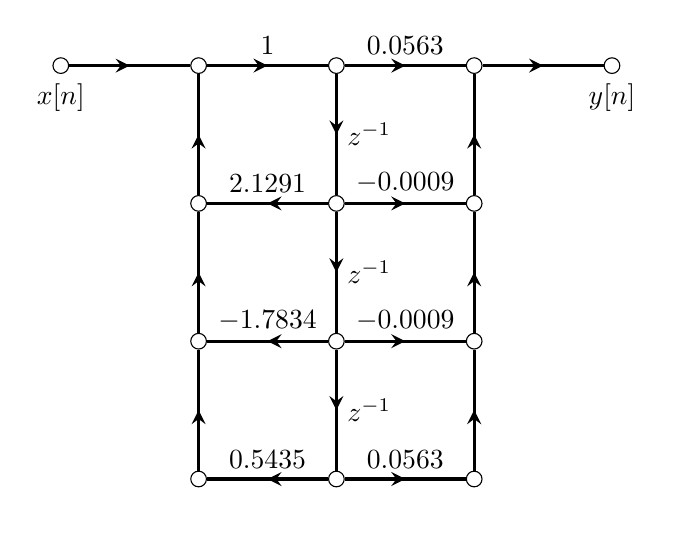
\begin{tikzpicture}[node distance=1.75cm]
%Place the nodes
\node[terminal={below}{$x[n]$}] (x) at (0,0) {};
\node[terminal={below}{}, right of=x] (00) {};
\node[terminal={below}{}, right of= 00] (01) {};
\node[terminal={below}{}, right of=01] (02) {};
\node[terminal={below}{$y[n]$}, right of=02] (y) {};

\foreach \j in {1, 2, 3} {
	\pgfmathtruncatemacro{\jn}{(\j-1)}%
	\node[terminal={below}{}, below of=\jn0] (\j0) {};
	\node[terminal={below}{}, below of=\jn1] (\j1) {};
	\node[terminal={below}{}, below of=\jn2] (\j2) {};
}

%
\draw[zpath={right}] (01) to (11);
\draw[zpath={right}] (11) to (21);
\draw[zpath={right}] (21) to (31);

%
\draw[amark] (10) to (00);
\draw[amark] (20) to (10);
\draw[amark] (30) to (20);

%
\draw[amark] (12) to (02);
\draw[amark] (22) to (12);
\draw[amark] (32) to (22);


%
\draw[amark={$1$}{above}] (00) to (01);
\draw[amark={$2.1291$}{above}] (11) to (10);
\draw[amark={$-1.7834$}{above}] (21) to (20);
\draw[amark={$0.5435$}{above}] (31) to (30);

%
\draw[amark={$0.0563$}{above}] (01) to (02);
\draw[amark={$-0.0009$}{above}] (11) to (12);
\draw[amark={$-0.0009$}{above}] (21) to (22);
\draw[amark={$0.0563$}{above}] (31) to (32);


\draw[amark] (x) to (00);
\draw[amark] (02) to (y);

\end{tikzpicture}}
\end{figure}
\FloatBarrier

\noindent\textbf{Notation warning:} the coefficients corresponding to the poles appear with a different sign.
\subsection{(c)}

\FloatBarrier
\begin{figure}[h!]
	\centering
	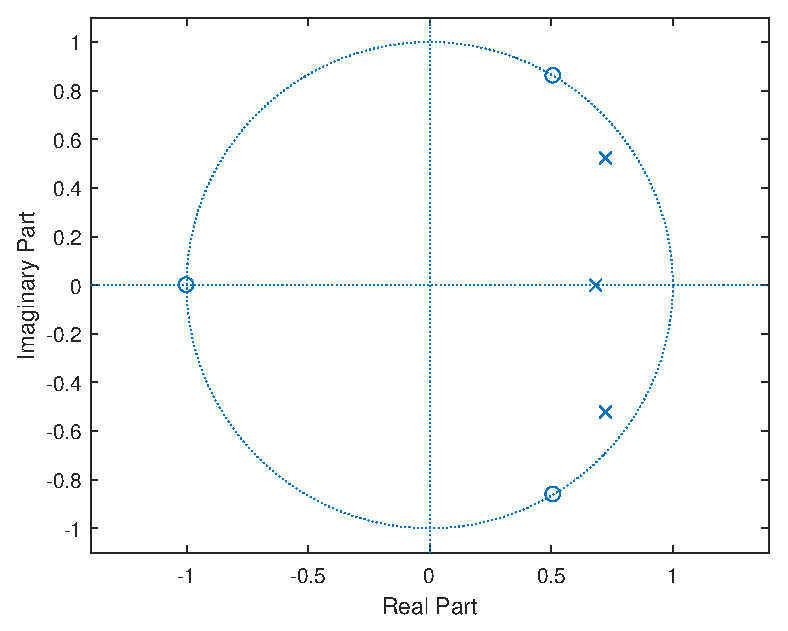
\includegraphics[scale=0.7]{figs/hw04q6_zplane.eps}
	\caption{Pole-zero diagram of $H(z)$.}
\end{figure}
\FloatBarrier

\subsection{(d)}

\FloatBarrier
\begin{figure}[h!]
	\centering
	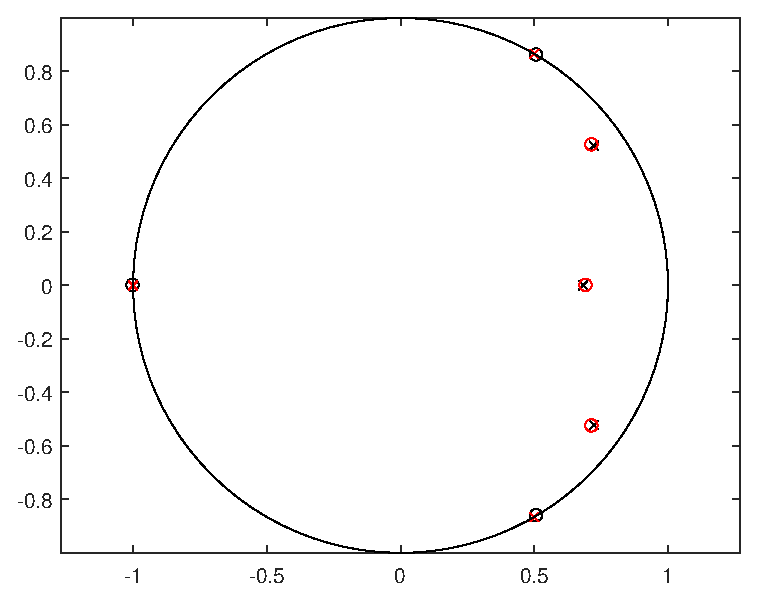
\includegraphics[scale=0.7]{figs/hw04q6_zplane_quant.eps}
	\caption{Comparison of pole-zero diagram of $H(z)$ before and after coefficient quantization.}
\end{figure}
\FloatBarrier

\FloatBarrier
\begin{figure}[h!]
	\centering
	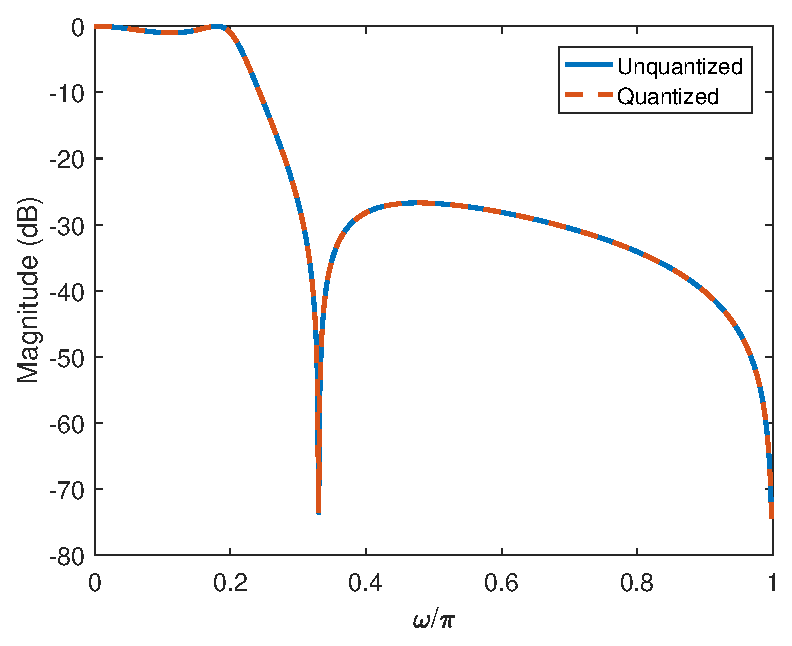
\includegraphics[scale=0.7]{figs/hw04q6_mag.eps}
	\caption{Comparison of magnitude response of $H(z)$ before and after coefficient quantization.}
\end{figure}
\FloatBarrier

The pole-zero diagram shows that the poles and zeros did not change much, and consequently all other properties of the system should remain roughly the same.


\newpage
\section{Problem 2}

\subsection{(a)}
By inspection
\begin{equation}
	H(z) = \frac{z^{-1} - a}{1 - az^{-1}}
\end{equation}

\subsection{(b)}

\begin{equation}
\sigma_{15}^2 = \frac{\Delta^2}{12} = \frac{2^{-30}}{12}
\end{equation}

\begin{figure}[!h]
	\centering
	\resizebox{0.5\textwidth}{!}{
\begin{tikzpicture}[node distance=1.75cm]
\tikzstyle{node}=[red2, circle,fill=red2,minimum size=2pt,inner sep=0pt]

\node[terminal={below}{$x[n]$}] (x) at (0,0) {};
\node[terminal={below}{}, right of=x] (00) {};
\node[terminal={below}{}, right of= 00] (01) {};
\node[terminal={below}{}, right of=01] (02) {};
\node[terminal={below}{$y[n]$}, right of=02] (y) {};

\coordinate[below of=00] (10) {};
\node[terminal={below}{}, below of=01] (11) {};
\coordinate[below of=02] (12) {};

%
\draw[zpath={right}] (11) to (01);

%
\draw[solid, \thickness] (00) to (10);
\draw[solid, \thickness] (02) to (12);
%

%
\draw[amark={$-a$}{above}] (00) to (01);
\draw[amark={$1$}{above}] (10) to (11);

%
\draw[amark={$1$}{above}] (01) to (02);
\draw[amark={$a$}{above}] (12) to (11);

\draw[amark] (x) to (00);
\draw[amark] (02) to (y);
\node[black, fill=black!10, below=1.5cm of y] {(A)}; 

\node[node, above=0.5cm of 01] (e0) {}; \node[right, red2] at (e0) {$\sigma_{15}^2$};
\draw[->, >=stealth, red2, \thickness] (e0) to (01);
\node[node, below=0.5cm of 11] (e1) {}; \node[right, red2] at (e1) {$\sigma_{15}^2$};
\draw[->, >=stealth, red2, \thickness] (e1) to (11);

\end{tikzpicture}
}

\resizebox{0.5\textwidth}{!}{
\begin{tikzpicture}[node distance=1.75cm]
\tikzstyle{node}=[red2, circle,fill=red2,minimum size=2pt,inner sep=0pt]

\node[terminal={below}{$x[n]$}] (x) at (0,0) {};
\node[terminal={below}{}, right=1cm of x] (00) {};
\node[terminal={below}{}, right=1.25cm of 00] (01) {};
\node[terminal={below}{}, right=1cm of 01] (02) {};
\node[terminal={below}{}, right=1.25cm of 02] (03) {};
\node[terminal={below}{$y[n]$}, right=1cm of 03] (y) {};

\node[terminal={below}{}, below of=00] (10) {};
\coordinate[below of=01] (11) {};
\coordinate[below of=02] (12) {};
\node[terminal={below}{}, below of=03] (13) {};

%
\draw[zpath={left}] (00) to (10);
\draw[amark={$1$}{below}] (10) to (11);
\draw[solid, \thickness] (11) to (01);

%
\draw[zpath={right}] (03) to (13);
\draw[amark={$a$}{below}] (13) to (12);
\draw[solid, \thickness] (12) to (02);

%
\draw[amark={}{right}] (x) to (00);
\draw[amark={$-a$}{above}] (00) to (01);
\draw[amark={}{right}] (01) to (02);
\draw[amark={}{right}] (03) to (y);

\draw[amark={$1$}{above}] (02) to (03);


\node[black, fill=black!10, below=1.5cm of y] {(B)}; 

\node[node, above=0.5cm of 01] (e0) {}; \node[right, red2] at (e0) {$\sigma_{15}^2$};
\draw[->, >=stealth, red2, \thickness] (e0) to (01);
\node[node, above=0.5cm of 02] (e1) {}; \node[right, red2] at (e1) {$\sigma_{15}^2$};
\draw[->, >=stealth, red2, \thickness] (e1) to (02);

\end{tikzpicture}
}

\resizebox{0.5\textwidth}{!}{
	\begin{tikzpicture}[node distance=1.75cm]
	\tikzstyle{node}=[red2, circle,fill=red2,minimum size=2pt,inner sep=0pt]
	\node[terminal={below}{$x[n]$}] (x) at (0,0) {};
	\node[terminal={below}{}, right of=x] (00) {};
	\node[terminal={below}{}, right of= 00] (01) {};
	\node[terminal={below}{}, right of=01] (02) {};
	\node[terminal={below}{$y[n]$}, right of=02] (y) {};
	
	\coordinate[below of=00] (10) {};
	\node[terminal={below}{}, below of=01] (11) {};
	\coordinate[below of=02] (12) {};
	
	%
	\draw[amark={$a$}{right}] (11) to (01);
	
	%
	\draw[solid, \thickness] (00) to (10);
	\draw[solid, \thickness] (02) to (12);
	%
	
	%
	\draw[amark={$z^{-1}$}{above}] (00) to (01);
	\draw[amark={$-1$}{above}] (10) to (11);
	
	%
	\draw[amark={$1$}{above}] (01) to (02);
	\draw[amark={$z^{-1}$}{above}] (12) to (11);
	
	\draw[amark] (x) to (00);
	\draw[amark] (02) to (y);
	\node[black, fill=black!10, below=1.5cm of y] {(C)}; 
	
	\node[node, above=0.5cm of 01] (e0) {}; \node[right, red2] at (e0) {$\sigma_{15}^2$};
	\draw[->, >=stealth, red2, \thickness] (e0) to (01);
	\end{tikzpicture}
}

\resizebox{0.5\textwidth}{!}{
	\begin{tikzpicture}[node distance=1.75cm]
	\tikzstyle{node}=[red2, circle,fill=red2,minimum size=2pt,inner sep=0pt]
	\node[terminal={below}{$x[n]$}] (x) at (0,0) {};
	\node[terminal={below}{}, right of=x] (00) {};
	\node[terminal={below}{}, right of= 00] (01) {};
	\node[terminal={below}{}, right of=01] (02) {};
	\node[terminal={below}{$y[n]$}, right of=02] (y) {};
	
	\coordinate[below of=00] (10) {};
	\node[terminal={below}{}, below of=01] (11) {};
	\coordinate[below of=02] (12) {};
	
	%
	\draw[amark={$z^{-1}$}{right}] (01) to (11);
	
	%
	\draw[solid, \thickness] (00) to (10);
	\draw[solid, \thickness] (02) to (12);
	%
	
	%
	\draw[amark={$1$}{above}] (00) to (01);
	\draw[amark={$a$}{above}] (11) to (10);
	
	%
	\draw[amark={$-a$}{above}] (01) to (02);
	\draw[amark={$1$}{above}] (11) to (12);
	
	\draw[amark] (x) to (00);
	\draw[amark] (02) to (y);
	\node[black, fill=black!10, below=1.5cm of y] {(D)}; 
	
	\node[node, above=0.5cm of 00] (e0) {}; \node[right, red2] at (e0) {$\sigma_{15}^2$};
	\draw[->, >=stealth, red2, \thickness] (e0) to (00);
	\node[node, above=0.5cm of 02] (e1) {}; \node[right, red2] at (e1) {$\sigma_{15}^2$};
	\draw[->, >=stealth, red2, \thickness] (e1) to (02);
	\end{tikzpicture}
}
\end{figure}

\subsection{(c)}

\begin{equation}
\Phi_{ff}(e^{j\omega}) = 2\sigma_{15}^2\bigg|\frac{1}{1-ae^{-j\omega}}\bigg|^2 = \frac{2\sigma_{15}^2}{1 + a^2 - 2a\cos\omega} \tag{(A)}
\end{equation}

\begin{equation}
\Phi_{ff}(e^{j\omega}) = 2\sigma_{15}^2\bigg|\frac{1}{1-ae^{-j\omega}}\bigg|^2 = \frac{2\sigma_{15}^2}{1 + a^2 - 2a\cos\omega} \tag{(B)}
\end{equation}

\begin{equation}
\Phi_{ff}(e^{j\omega}) = \sigma_{15}^2\bigg|\frac{1}{1-ae^{-j\omega}}\bigg|^2 = \frac{\sigma_{15}^2}{1 + a^2 - 2a\cos\omega} \tag{(C)}
\end{equation}

\begin{equation}
\Phi_{ff}(e^{j\omega}) = \sigma_{15}^2 + \sigma_{15}^2|H(e^{j\omega})|^2 = 2\sigma_{15}^2 \tag{(D)}
\end{equation}

\subsection{(d)}

(A) and (B) will have the largest output noise average power.

\begin{equation}
	\sigma_{f}^2 = 2\sigma_{15}^2\sum_{k = 0}^\infty (a^2)^k = \frac{2\sigma_{15}^2}{1 - a^2}
\end{equation}

The above equation comes from computing the inverse DTFT of the PSD found in part (c), which is a a typical second-order transform. 

Note: It can be shown that (A) and (B) will have the largest output noise by showing that the integral of the PSD is larger in those systems. 	
	
\newpage
\section{Problem 3}

Matlab code for this problem is attached at the end of this question.

\subsection{(a)}

The parameters of the filters are listed below
\begin{itemize}
	\item 3-dB bandwidth or cut-off frequency: 4 kHz, which for $1/T = 16$ kHz corresponds to $\omega_c = \pi/2$ 
	\item Order: 8
	\item Ripple (only used in Chebyshev I and elliptic filters): 1 dB, any other answer is acceptable. However, the ripple in the passband cannot be very large.
	\item Stopband edge frequency (only used in Chebyshev II and elliptic filters): $1.1\omega_c$. This value led to a cutoff frequency of nearly 4 kHz. Other answer are accepted, as long as the cutoff frequency is close to 4 kHz
	\item Stopband attenuation (only used in Chebyshev II and elliptic filters): 30 dB. Other answers are accepted.
\end{itemize}

\FloatBarrier
\begin{figure}[h!]
	\centering
	\begin{subfigure}[h!]{0.5\textwidth}
		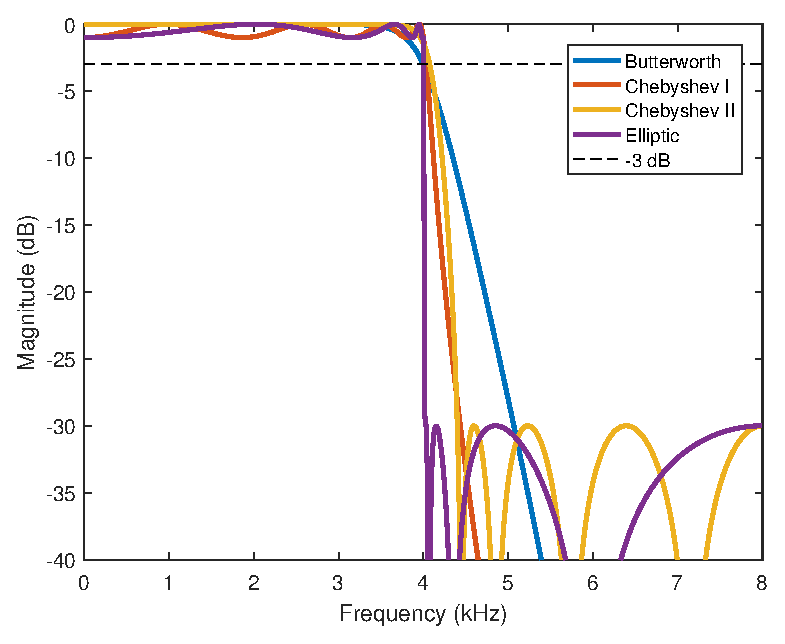
\includegraphics[width=\textwidth]{figs/classic_filters_mag.eps}
		\caption{Magnitude}
		\label{fig:mag}
	\end{subfigure}%
	~
	\begin{subfigure}[h!]{0.5\textwidth}
		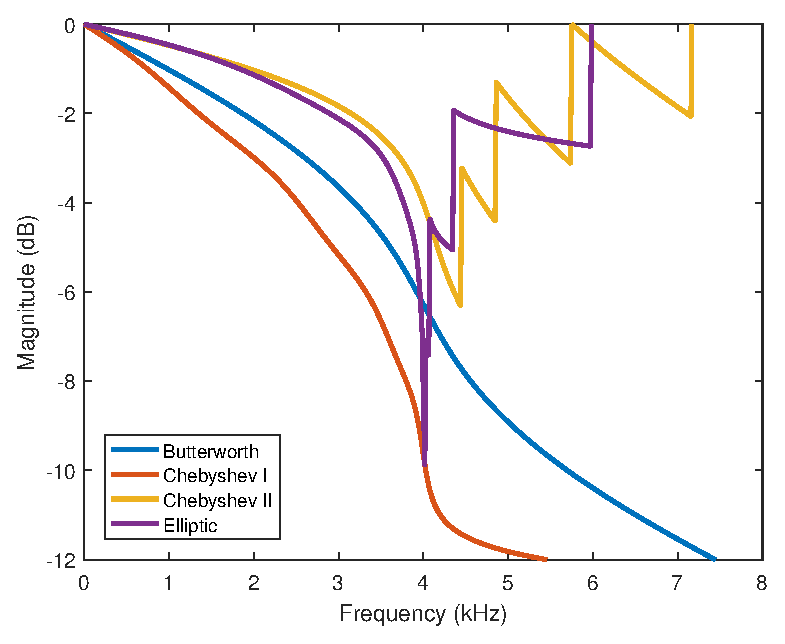
\includegraphics[width=\textwidth]{figs/classic_filters_phase.eps}
		\caption{Phase}
		\label{fig:phase}
	\end{subfigure}
	\caption{(a) Magnitude and (b) phase responses of the filters designed.}\label{fig:q81a}
\end{figure}

\FloatBarrier

\subsection{(b)}

See Matlab code for solution to this question.

To achieve the desired non-integer sampling rate change, we must upsample by 320 and decimate by 441.

One comment regarding implementation is that the lowpass filter between the upsampling and downsampling stages must have gain $L$. However, the lowpass filter prior to downsampling in decimation (and in the \texttt{decimate} function) has gain 1. Therefore, we must scale the result by $L$. For more details, refer to slide 30 of lecture notes 4.

\subsection{(c)}

This problem is equivalent to interchanging decimation and filtering. Therefore, it follows that
\begin{equation}
	H_{32}(z) = H_{16}(z^2)
\end{equation}

\subsection{Matlab code for Problem 3}

% This file was automatically created from the m-file 
% "m2tex.m" written by USL. 
% The fontencoding in this file is UTF-8. 
%  
% You will need to include the following two packages in 
% your LaTeX-Main-File. 
%  
% \usepackage{color} 
% \usepackage{fancyvrb} 
%  
% It is advised to use the following option for Inputenc 
% \usepackage[utf8]{inputenc} 
%  
  
% definition of matlab colors: 
\definecolor{mblue}{rgb}{0,0,1} 
\definecolor{mgreen}{rgb}{0.13333,0.5451,0.13333} 
\definecolor{mred}{rgb}{0.62745,0.12549,0.94118} 
\definecolor{mgrey}{rgb}{0.5,0.5,0.5} 
\definecolor{mdarkgrey}{rgb}{0.25,0.25,0.25} 
  
\DefineShortVerb[fontfamily=courier,fontseries=m]{\$} 
\DefineShortVerb[fontfamily=courier,fontseries=b]{\#} 
  
\noindent                                                                                      
 \hspace*{-1.6em}{\scriptsize 1}$  $\color{mgrey}#%% Comparison of famous filters#\color{black}$$\\
 \hspace*{-1.6em}{\scriptsize 2}$  clear, $\color{mdarkgrey}$clc, close all$\color{black}$$\\
 \hspace*{-1.6em}{\scriptsize 3}$  $\\
 \hspace*{-1.6em}{\scriptsize 4}$  $\color{mgrey}#%% a) Design filters#\color{black}$$\\
 \hspace*{-1.6em}{\scriptsize 5}$  N = 8;                      $\color{mgrey}$% filter order$\color{black}$$\\
 \hspace*{-1.6em}{\scriptsize 6}$  wc = pi/2;                  $\color{mgrey}$% cutoff frequency wc = 2pi*4/16 = pi/2$\color{black}$$\\
 \hspace*{-1.6em}{\scriptsize 7}$  Rp = 1;                     $\color{mgrey}$% pass-band ripple$\color{black}$$\\
 \hspace*{-1.6em}{\scriptsize 8}$  ws = 1.1*wc;                $\color{mgrey}$% stopband edge frequency to achieve wc = 4 kHz$\color{black}$$\\
 \hspace*{-1.6em}{\scriptsize 9}$  Rs = 30;                    $\color{mgrey}$% stopband attenuation$\color{black}$$\\
 \hspace*{-2em}{\scriptsize 10}$  T = 1/16e3;                 $\color{mgrey}$% sampling period$\color{black}$$\\
 \hspace*{-2em}{\scriptsize 11}$  $\\
 \hspace*{-2em}{\scriptsize 12}$  $\color{mgrey}$% Design filters$\color{black}$$\\
 \hspace*{-2em}{\scriptsize 13}$  [num_butter, $\color{mdarkgrey}$den_butter] = butter(N, wc/pi);$\color{black}$$\\
 \hspace*{-2em}{\scriptsize 14}$  [num_cheby1, $\color{mdarkgrey}$den_cheby1] = cheby1(N, Rp, wc/pi);$\color{black}$$\\
 \hspace*{-2em}{\scriptsize 15}$  [num_cheby2, $\color{mdarkgrey}$den_cheby2] = cheby2(N, Rs, ws/pi);$\color{black}$$\\
 \hspace*{-2em}{\scriptsize 16}$  [num_ellip, $\color{mdarkgrey}$den_ellip] = ellip(N, Rp, Rs, wc/pi);$\color{black}$$\\
 \hspace*{-2em}{\scriptsize 17}$  $\\
 \hspace*{-2em}{\scriptsize 18}$  $\color{mgrey}$% Frequency response$\color{black}$$\\
 \hspace*{-2em}{\scriptsize 19}$  [H_butter, $\color{mdarkgrey}$w] = freqz(num_butter, den_butter);$\color{black}$$\\
 \hspace*{-2em}{\scriptsize 20}$  H_cheby1 = freqz(num_cheby1, den_cheby1, w);$\\
 \hspace*{-2em}{\scriptsize 21}$  H_cheby2 = freqz(num_cheby2, den_cheby2, w);$\\
 \hspace*{-2em}{\scriptsize 22}$  H_ellip = freqz(num_ellip, den_ellip, w);$\\
 \hspace*{-2em}{\scriptsize 23}$  $\\
 \hspace*{-2em}{\scriptsize 24}$  $\color{mgrey}$% Pole-zero$\color{black}$$\\
 \hspace*{-2em}{\scriptsize 25}$  figure, $\color{mdarkgrey}$zplane(num_butter, den_butter)$\color{black}$$\\
 \hspace*{-2em}{\scriptsize 26}$  figure, $\color{mdarkgrey}$zplane(num_cheby1, den_cheby1)$\color{black}$$\\
 \hspace*{-2em}{\scriptsize 27}$  figure, $\color{mdarkgrey}$zplane(num_cheby2, den_cheby2)$\color{black}$$\\
 \hspace*{-2em}{\scriptsize 28}$  figure, $\color{mdarkgrey}$zplane(num_ellip, den_ellip)$\color{black}$$\\
 \hspace*{-2em}{\scriptsize 29}$  $\\
 \hspace*{-2em}{\scriptsize 30}$  $\color{mgrey}$% Plot results$\color{black}$$\\
 \hspace*{-2em}{\scriptsize 31}$  figure, $\color{mdarkgrey}$hold on, box on$\color{black}$$\\
 \hspace*{-2em}{\scriptsize 32}$  plot(w/(2*pi*T)*1e-3, $\color{mdarkgrey}$20*log10(abs(H_butter)),...$\color{black}$$\\
 \hspace*{-2em}{\scriptsize 33}$      $\color{mdarkgrey}$'LineWidth'$\color{black}$, 2, $\color{mdarkgrey}$'displayName'$\color{black}$, $\color{mdarkgrey}$'Butterworth'$\color{black}$)$\\
 \hspace*{-2em}{\scriptsize 34}$  plot(w/(2*pi*T)*1e-3, $\color{mdarkgrey}$20*log10(abs(H_cheby1)),...$\color{black}$$\\
 \hspace*{-2em}{\scriptsize 35}$      $\color{mdarkgrey}$'LineWidth'$\color{black}$, 2, $\color{mdarkgrey}$'displayName'$\color{black}$, $\color{mdarkgrey}$'Chebyshev I'$\color{black}$)$\\
 \hspace*{-2em}{\scriptsize 36}$  plot(w/(2*pi*T)*1e-3, $\color{mdarkgrey}$20*log10(abs(H_cheby2)),...$\color{black}$$\\
 \hspace*{-2em}{\scriptsize 37}$      $\color{mdarkgrey}$'LineWidth'$\color{black}$, 2, $\color{mdarkgrey}$'displayName'$\color{black}$, $\color{mdarkgrey}$'Chebyshev II'$\color{black}$)$\\
 \hspace*{-2em}{\scriptsize 38}$  plot(w/(2*pi*T)*1e-3, $\color{mdarkgrey}$20*log10(abs(H_ellip)),...$\color{black}$$\\
 \hspace*{-2em}{\scriptsize 39}$  $\color{mdarkgrey}$'LineWidth'$\color{black}$, 2, $\color{mdarkgrey}$'displayName'$\color{black}$, $\color{mdarkgrey}$'Elliptic'$\color{black}$)$\\
 \hspace*{-2em}{\scriptsize 40}$  plot([0 1e-3/T], [-3 -3], $\color{mdarkgrey}$'--k'$\color{black}$, $\color{mdarkgrey}$'DisplayName'$\color{black}$, $\color{mdarkgrey}$'-3 dB'$\color{black}$)$\\
 \hspace*{-2em}{\scriptsize 41}$  xlabel($\color{mdarkgrey}$'Frequency (kHz)'$\color{black}$)$\\
 \hspace*{-2em}{\scriptsize 42}$  ylabel($\color{mdarkgrey}$'Magnitude (dB)'$\color{black}$)$\\
 \hspace*{-2em}{\scriptsize 43}$  axis([0 $\color{mdarkgrey}$0.5e-3/T -40 0])$\color{black}$$\\
 \hspace*{-2em}{\scriptsize 44}$  legend($\color{mdarkgrey}$'-dynamiclegend'$\color{black}$)$\\
 \hspace*{-2em}{\scriptsize 45}$  saveas(gca, $\color{mdarkgrey}$'../figs/classic_filters_mag'$\color{black}$, $\color{mdarkgrey}$'epsc'$\color{black}$)$\\
 \hspace*{-2em}{\scriptsize 46}$  $\\
 \hspace*{-2em}{\scriptsize 47}$  figure, $\color{mdarkgrey}$hold on, box on$\color{black}$$\\
 \hspace*{-2em}{\scriptsize 48}$  plot(w/(2*pi*T)*1e-3, $\color{mdarkgrey}$unwrap(angle(H_butter)),...$\color{black}$$\\
 \hspace*{-2em}{\scriptsize 49}$      $\color{mdarkgrey}$'LineWidth'$\color{black}$, 2, $\color{mdarkgrey}$'displayName'$\color{black}$, $\color{mdarkgrey}$'Butterworth'$\color{black}$)$\\
 \hspace*{-2em}{\scriptsize 50}$  plot(w/(2*pi*T)*1e-3, $\color{mdarkgrey}$unwrap(angle(H_cheby1)),...$\color{black}$$\\
 \hspace*{-2em}{\scriptsize 51}$      $\color{mdarkgrey}$'LineWidth'$\color{black}$, 2, $\color{mdarkgrey}$'displayName'$\color{black}$, $\color{mdarkgrey}$'Chebyshev I'$\color{black}$)$\\
 \hspace*{-2em}{\scriptsize 52}$  plot(w/(2*pi*T)*1e-3, $\color{mdarkgrey}$unwrap(angle(H_cheby2)),...$\color{black}$$\\
 \hspace*{-2em}{\scriptsize 53}$      $\color{mdarkgrey}$'LineWidth'$\color{black}$, 2, $\color{mdarkgrey}$'displayName'$\color{black}$, $\color{mdarkgrey}$'Chebyshev II'$\color{black}$)$\\
 \hspace*{-2em}{\scriptsize 54}$  plot(w/(2*pi*T)*1e-3, $\color{mdarkgrey}$unwrap(angle(H_ellip)),...$\color{black}$$\\
 \hspace*{-2em}{\scriptsize 55}$      $\color{mdarkgrey}$'LineWidth'$\color{black}$, 2, $\color{mdarkgrey}$'displayName'$\color{black}$, $\color{mdarkgrey}$'Elliptic'$\color{black}$)$\\
 \hspace*{-2em}{\scriptsize 56}$  legend($\color{mdarkgrey}$'-dynamiclegend'$\color{black}$, $\color{mdarkgrey}$'Location'$\color{black}$, $\color{mdarkgrey}$'SouthWest'$\color{black}$)$\\
 \hspace*{-2em}{\scriptsize 57}$  xlabel($\color{mdarkgrey}$'Frequency (kHz)'$\color{black}$)$\\
 \hspace*{-2em}{\scriptsize 58}$  ylabel($\color{mdarkgrey}$'Magnitude (dB)'$\color{black}$)$\\
 \hspace*{-2em}{\scriptsize 59}$  axis([0 $\color{mdarkgrey}$0.5e-3/T -12 0])$\color{black}$$\\
 \hspace*{-2em}{\scriptsize 60}$  saveas(gca, $\color{mdarkgrey}$'../figs/classic_filters_phase'$\color{black}$, $\color{mdarkgrey}$'epsc'$\color{black}$)$\\
 \hspace*{-2em}{\scriptsize 61}$  $\\
 \hspace*{-2em}{\scriptsize 62}$  $\color{mgrey}#%% b) Filter speech#\color{black}$$\\
 \hspace*{-2em}{\scriptsize 63}$  $\color{mgrey}$% Load speech signal$\color{black}$$\\
 \hspace*{-2em}{\scriptsize 64}$  [x_orig, Fs] = audioread($\color{mdarkgrey}$'speech_dft.wav'$\color{black}$);          $\color{mgrey}$% Fs is sampling frequency$\color{black}$$\\
 \hspace*{-2em}{\scriptsize 65}$  T = 1/Fs;                                            $\color{mgrey}$% sampling period$\color{black}$$\\
 \hspace*{-2em}{\scriptsize 66}$  $\\
 \hspace*{-2em}{\scriptsize 67}$  $\color{mgrey}$% Express 16/22.05 as fraction L/M$\color{black}$$\\
 \hspace*{-2em}{\scriptsize 68}$  [L, $\color{mdarkgrey}$M] = rat(16/22.05); $\color{black}$$\color{mgrey}$% L is the umpsampling factor and M is the downsampling factor$\color{black}$$\\
 \hspace*{-2em}{\scriptsize 69}$         $\\
 \hspace*{-2em}{\scriptsize 70}$  $\color{mgrey}#%% Upsampling followed by decimation.#\color{black}$$\\
 \hspace*{-2em}{\scriptsize 71}$  $\color{mgrey}$% Note that the lowpass filter between the upsampling and downsampling $\color{black}$$\\
 \hspace*{-2em}{\scriptsize 72}$  $\color{mgrey}$% stages must have gain L. However, the lowpass filter prior to $\color{black}$$\\
 \hspace*{-2em}{\scriptsize 73}$  $\color{mgrey}$% downsampling in decimation (and in the decimate function) has gain 1.$\color{black}$$\\
 \hspace*{-2em}{\scriptsize 74}$  $\color{mgrey}$% Therefore, we must scale the result by L$\color{black}$$\\
 \hspace*{-2em}{\scriptsize 75}$  $\color{mgrey}$% For more details, refer to slide 30 of lecture notes 4.$\color{black}$$\\
 \hspace*{-2em}{\scriptsize 76}$  x = L*decimate(upsample(x_orig, L), M);$\\
 \hspace*{-2em}{\scriptsize 77}$  Fs = 16e3;  $\color{mgrey}$% Sampling rate after upsampling/decimation$\color{black}$$\\
 \hspace*{-2em}{\scriptsize 78}$  $\\
 \hspace*{-2em}{\scriptsize 79}$  y_butter = filter(num_butter, den_butter, x);$\\
 \hspace*{-2em}{\scriptsize 80}$  y_cheby1 = filter(num_cheby1, den_cheby1, x);$\\
 \hspace*{-2em}{\scriptsize 81}$  y_cheby2 = filter(num_cheby2, den_cheby2, x);$\\
 \hspace*{-2em}{\scriptsize 82}$  y_ellip = filter(num_ellip, den_ellip, x);$\\
 \hspace*{-2em}{\scriptsize 83}$  $\\
 \hspace*{-2em}{\scriptsize 84}$  sound(y_ellip, $\color{mdarkgrey}$Fs) $\color{black}$$\color{mgrey}$% play sound after filtering$\color{black}$$\\
 \hspace*{-2em}{\scriptsize 85}$  $\\
 \hspace*{-2em}{\scriptsize 86}$  $\\ 
  
\UndefineShortVerb{\$} 
\UndefineShortVerb{\#}

\newpage
\section{Problem 4}

Matlab code for this problem is attached at the end of this question.

\subsection{(a)}

For $\lambda$ there's only one choice: $\lambda = 2\pi60 = 120\pi$.

The parameter $b$ controls the sharpness of the notch (loosely the so-called $Q$ factor). We would like to make $b$ smaller as possible, but this would reduce the attenuation of the notch. A reasonable choice is $b = 2\pi 5 = 10\pi$. This allows reasonable sharpness with enough attenuation. Other reasonable answers are accepted.

\subsection{(b)}

For this we just can use the \texttt{bilinear} function from Matlab. The frequency pre-warping frequency must be $\Omega_p = \lambda$ so that the location of the notch is preserved when converting the filter to discrete time.
\begin{align*}
	&\texttt{>> [bzw, azw] = bilinear(bs, as, 1/T);} \tag{without frequency pre-warping} \\
	&\texttt{>> [bz, az] = bilinear(bs, as, 1/T, lamb/(2*pi));} \tag{with frequency pre-warping}
\end{align*}

See code for context.

\subsection{(c)}

From Figure~\ref{fig:egc:bilinear-mag} we clearly see that we must use frequency pre-warping, otherwise the frequency of the notch would shift, and consequently the filter would no longer be suitable to remove the 60 Hz interference. 

\FloatBarrier
\begin{figure}[h!]
	\centering
	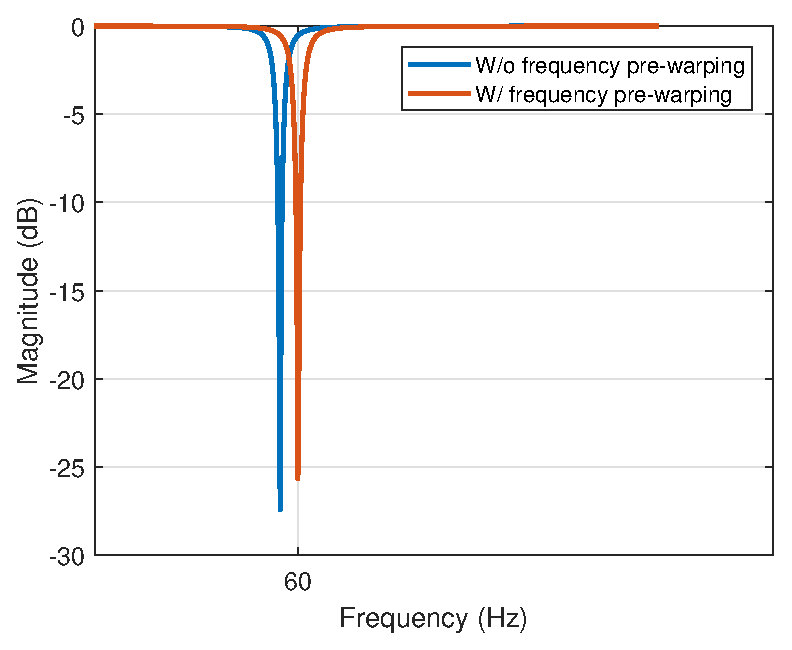
\includegraphics[scale=0.7]{figs/bilinear_ecg.eps}
	\caption{Magnitude response of digital filter obtained by bilinear transformation with and without frequency pre-warping.} \label{fig:egc:bilinear-mag}
\end{figure}
\FloatBarrier

\subsection{(d)}

From Figure~\ref{fig:egc:bilinear-mag} we see that $H(z)$ obtained with bilinear transformation has zeros at $e^{\pm j2\pi60T}$. These zeros are responsible for the notch in the magnitude response. The pole close to the zero guarantees that away from $60 Hz$ the magnitude response looks flat.  

\FloatBarrier
\begin{figure}[h!]
	\centering
	\includegraphics[scale=0.7]{figs/zplane_bilinear_ecg.eps}
	\caption{Pole-zero diagram of $H(z)$ obtained by bilinear transformation with frequency pre-warping.} \label{fig:egc:bilinear-zplane}
\end{figure}
\FloatBarrier

\subsection{(e)}

As shown in Figures~\ref{fig:egc:comparison1} and \ref{fig:egc:comparison2} the digital notch filter designed effectively eliminates the 60-Hz interference.

\FloatBarrier
\begin{figure}[h!]
	\centering
	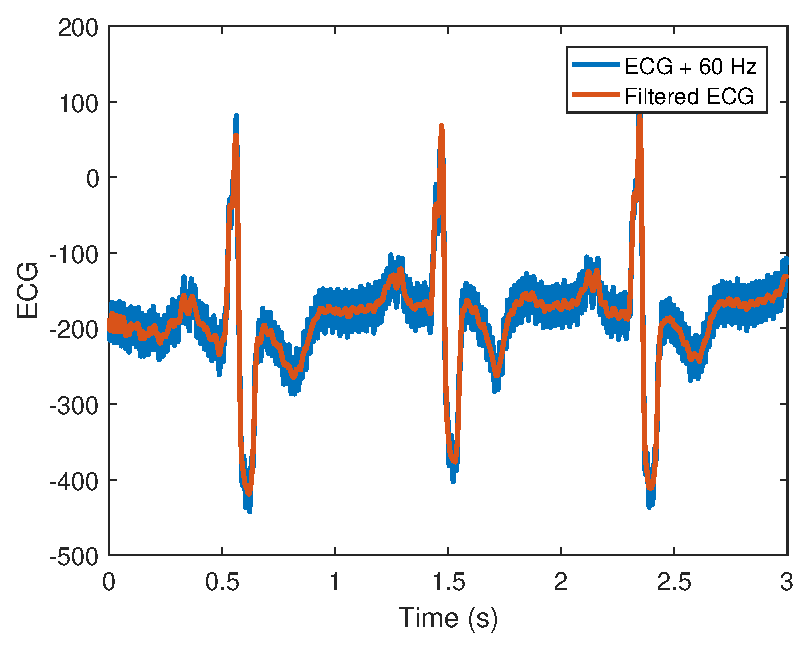
\includegraphics[scale=0.9]{figs/ecg_comparison1.eps}
	\caption{Comparison between digital notch filter input (ECG with 60 interference), and digital notch filter output.} \label{fig:egc:comparison1}
\end{figure}
\FloatBarrier

\FloatBarrier
\begin{figure}[h!]
	\centering
	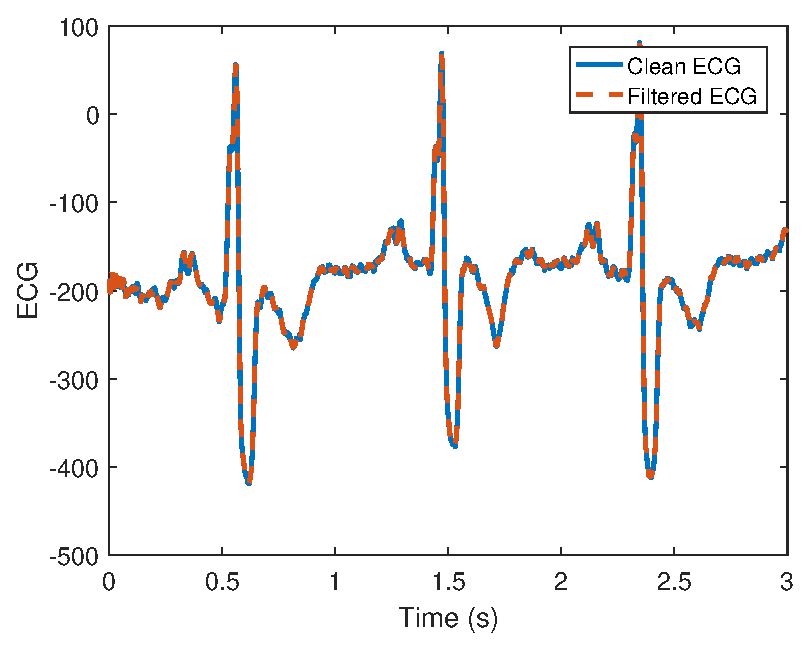
\includegraphics[scale=0.9]{figs/ecg_comparison2.eps}
	\caption{Comparison between digital ``clean'' ECG signal (ECG without 60 interference), and the digital notch filter output.} \label{fig:egc:comparison2}
\end{figure}
\FloatBarrier

\subsection{(f)}

Figure~\ref{fig:egc:fir_notch} shows the magnitude response of the designed FIR filter. The filter was optimized using the least-squares algorithm with the following design parameters:
\begin{itemize}
	\item Order: 52 the highest value allowed in the problem statement
	\item $\omega_cT = 2\pi 60 = 120\pi$. So that the notch falls at 60 Hz.
	\item $\Delta\omega_1 = 0.018\pi$. Other values are accepted.
	\item $\Delta\omega_2 = 0.04\pi$. Other values are accepted.
\end{itemize}
	
This filter has nice properties. It has a high attenuation of 55 dB in the notch, which is higher than the filter from part (c). Moreover, the notch is not too wide. Furthermore, the ripples in the passband are not significant.

The filter from the \href{http://ieeexplore.ieee.org/document/1351410/}{2004 paper} has higher attenuation at the cost of a wider notch and more ripples in the passband. Moreover, their filter was designed for a higher oversampling rate, which facilitates filtering. Their sampling rate was 1 kHz, while the sample rate of our signal was $\sim 333$ Hz.
	
\FloatBarrier
\begin{figure}[h!]
	\centering
	\begin{subfigure}[h!]{0.5\textwidth}
		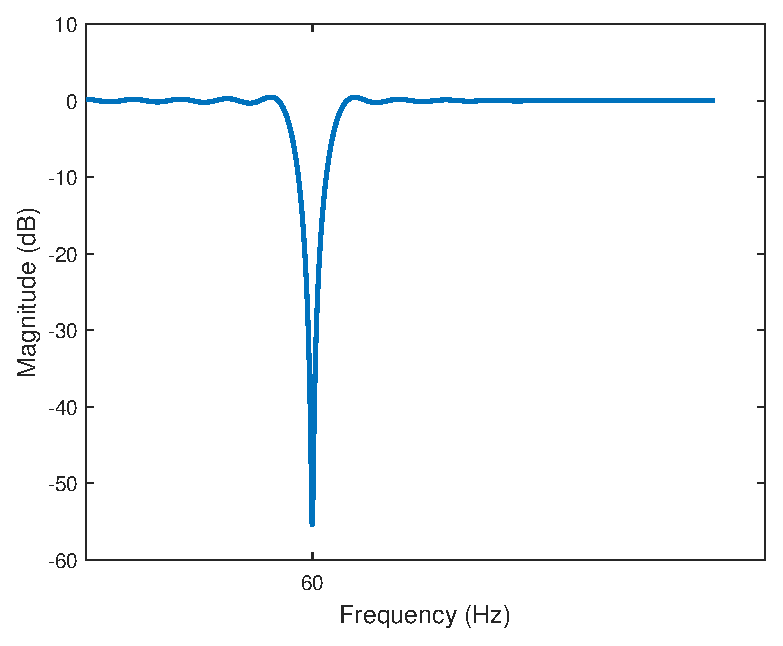
\includegraphics[width=\textwidth]{figs/ecg_fir_notch.eps}
		\caption{Magnitude response of FIR notch filter.} \label{fig:egc:fir_notch}
	\end{subfigure}%
	~ %add desired spacing between images, e. g. ~, \quad, \qquad etc.
	%(or a blank line to force the subfigure onto a new line)
	\begin{subfigure}[h!]{0.5\textwidth}
		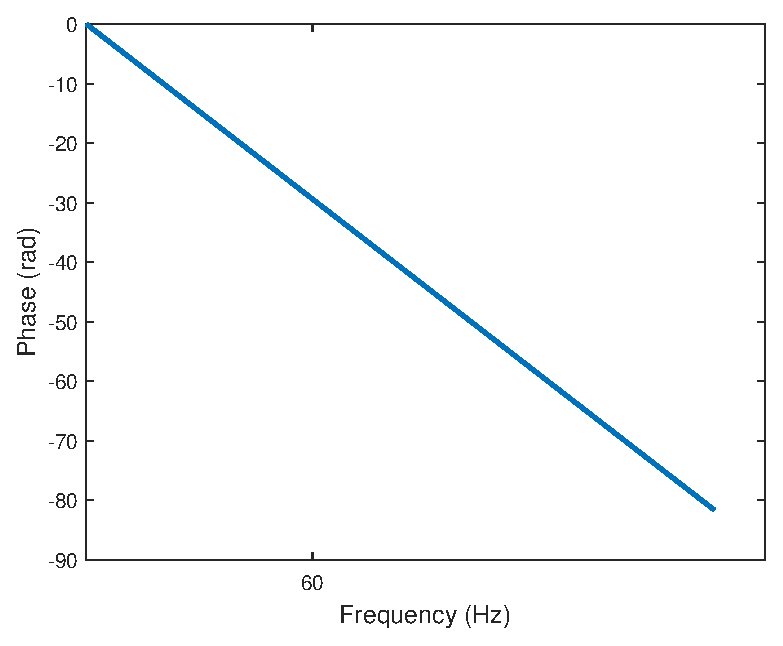
\includegraphics[width=\textwidth]{figs/ecg_fir_notch_phase.eps}
		\caption{Phase response of FIR notch filter.} \label{fig:egc:fir_notch_phase}
	\end{subfigure}
	\caption{(a) magnitude and (b) phase response of FIR notch filter.}
\end{figure}
\FloatBarrier

Due to the linear phase property, the FIR filter introduces a delay of $M/2 = 26$ samples. The plots below show the comparison of the FIR filter with the ``clean'' ECG with delay and without delay.

\FloatBarrier
\begin{figure}[h!]
	\centering
	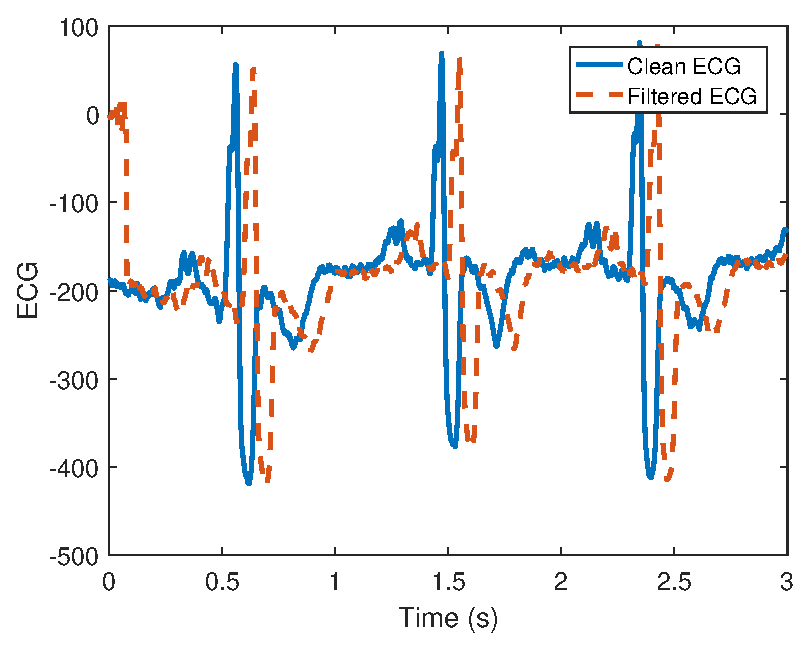
\includegraphics[scale=0.9]{figs/ecg_fir_comparison1.eps}
	\caption{Comparison between digital ``clean'' ECG signal (ECG without 60 interference), and the digital notch FIR filter output. In this case the delay introduced by the filter was not removed. } \label{fig:egc:fir_comparison1}
\end{figure}
\FloatBarrier

\FloatBarrier
\begin{figure}[h!]
	\centering
	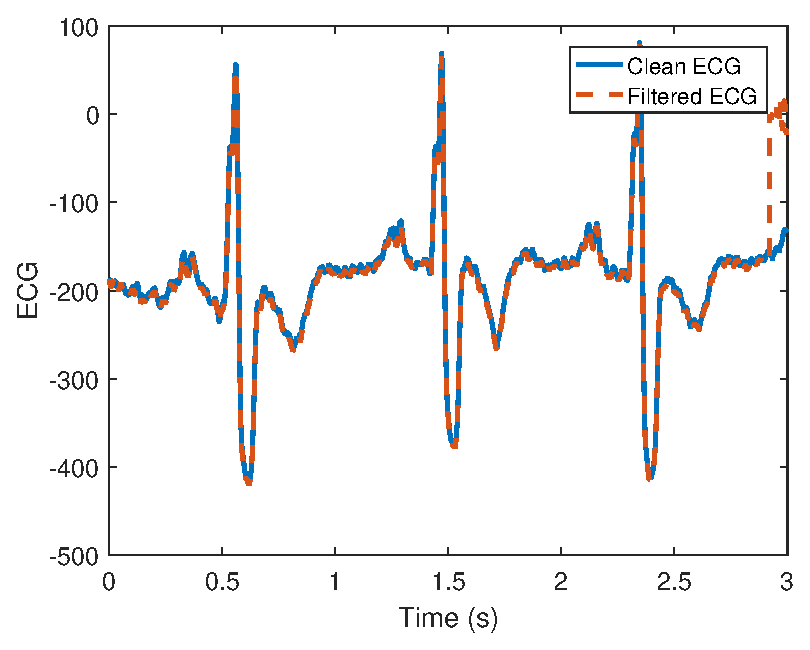
\includegraphics[scale=0.9]{figs/ecg_fir_comparison2.eps}
	\caption{Comparison between digital ``clean'' ECG signal (ECG without 60 interference), and the digital notch FIR filter output. Delay introduced by the FIR filter was removed.} \label{fig:egc:fir_comparison2}
\end{figure}
\FloatBarrier

\subsection{Matlab code for Problem 4}
% This file was automatically created from the m-file 
% "m2tex.m" written by USL. 
% The fontencoding in this file is UTF-8. 
%  
% You will need to include the following two packages in 
% your LaTeX-Main-File. 
%  
% \usepackage{color} 
% \usepackage{fancyvrb} 
%  
% It is advised to use the following option for Inputenc 
% \usepackage[utf8]{inputenc} 
%  
  
% definition of matlab colors: 
\definecolor{mblue}{rgb}{0,0,1} 
\definecolor{mgreen}{rgb}{0.13333,0.5451,0.13333} 
\definecolor{mred}{rgb}{0.62745,0.12549,0.94118} 
\definecolor{mgrey}{rgb}{0.5,0.5,0.5} 
\definecolor{mdarkgrey}{rgb}{0.25,0.25,0.25} 
  
\DefineShortVerb[fontfamily=courier,fontseries=m]{\$} 
\DefineShortVerb[fontfamily=courier,fontseries=b]{\#} 
  
\noindent                                                                                                                                                            
 \hspace*{-1.6em}{\scriptsize 1}$  $\color{mgrey}#%% Template for notch filtering of ECG signals#\color{black}$$\\
 \hspace*{-1.6em}{\scriptsize 2}$  clear, $\color{mdarkgrey}$clc, close all$\color{black}$$\\
 \hspace*{-1.6em}{\scriptsize 3}$  $\\
 \hspace*{-1.6em}{\scriptsize 4}$  $\color{mgrey}#%% Loads ECG signal from file#\color{black}$$\\
 \hspace*{-1.6em}{\scriptsize 5}$  $\color{mgrey}$% This loads the following variables:$\color{black}$$\\
 \hspace*{-1.6em}{\scriptsize 6}$  $\color{mgrey}$% - ecg_clean: ecg_signal without 60 Hz interference. Use this only for$\color{black}$$\\
 \hspace*{-1.6em}{\scriptsize 7}$  $\color{mgrey}$% comparison$\color{black}$$\\
 \hspace*{-1.6em}{\scriptsize 8}$  $\color{mgrey}$% - ecg_60Hz: ECG signal corrupted by 60 Hz interference$\color{black}$$\\
 \hspace*{-1.6em}{\scriptsize 9}$  $\color{mgrey}$% - N: length of the vectors ecg_clean and ecg_60Hz$\color{black}$$\\
 \hspace*{-2em}{\scriptsize 10}$  $\color{mgrey}$% - T (in seconds): sampling period of ECG recordings. T = 3 ms.$\color{black}$$\\
 \hspace*{-2em}{\scriptsize 11}$  load($\color{mdarkgrey}$'ecg_recording.mat'$\color{black}$) $\\
 \hspace*{-2em}{\scriptsize 12}$  $\color{mgrey}$% Note: these signals are real ECG recordings made with standard ECG recorders, $\color{black}$$\\
 \hspace*{-2em}{\scriptsize 13}$  $\color{mgrey}$% leads, and electrodes. The quality is typical of ambulatory ECG recordings.$\color{black}$$\\
 \hspace*{-2em}{\scriptsize 14}$  $\color{mgrey}$% The 60 Hz component was introduced artificially for this exercise.$\color{black}$$\\
 \hspace*{-2em}{\scriptsize 15}$  $\color{mgrey}$% The complete database can be found online on PhysioNet [1]: $\color{black}$$\\
 \hspace*{-2em}{\scriptsize 16}$  $\color{mgrey}$% http://www.physionet.org/physiobank/database/nstdb/$\color{black}$$\\
 \hspace*{-2em}{\scriptsize 17}$  $\color{mgrey}$% This database is discrebed in [2].$\color{black}$$\\
 \hspace*{-2em}{\scriptsize 18}$  $\color{mgrey}$% References:$\color{black}$$\\
 \hspace*{-2em}{\scriptsize 19}$  $\color{mgrey}$% [1] Goldberger AL, Amaral LAN, Glass L, Hausdorff JM, Ivanov PCh, Mark RG, $\color{black}$$\\
 \hspace*{-2em}{\scriptsize 20}$  $\color{mgrey}$% Mietus JE, Moody GB, Peng C-K, Stanley HE. PhysioBank, PhysioToolkit, and $\color{black}$$\\
 \hspace*{-2em}{\scriptsize 21}$  $\color{mgrey}$% PhysioNet: Components of a New Research Resource for Complex Physiologic $\color{black}$$\\
 \hspace*{-2em}{\scriptsize 22}$  $\color{mgrey}$% Signals. Circulation 101(23):e215-e220 [Circulation Electronic Pages; $\color{black}$$\\
 \hspace*{-2em}{\scriptsize 23}$  $\color{mgrey}$% http://circ.ahajournals.org/content/101/23/e215.full]; 2000 (June 13).$\color{black}$$\\
 \hspace*{-2em}{\scriptsize 24}$  $\color{mgrey}$% [2] Moody GB, Muldrow WE, Mark RG. A noise stress test for arrhythmia detectors. $\color{black}$$\\
 \hspace*{-2em}{\scriptsize 25}$  $\color{mgrey}$% Computers in Cardiology 1984; 11:381-384.$\color{black}$$\\
 \hspace*{-2em}{\scriptsize 26}$  $\\
 \hspace*{-2em}{\scriptsize 27}$  t = 0:T:(N-1)*T; $\color{mgrey}$% time vector$\color{black}$$\\
 \hspace*{-2em}{\scriptsize 28}$  $\\
 \hspace*{-2em}{\scriptsize 29}$  $\color{mgrey}$% Plot signals$\color{black}$$\\
 \hspace*{-2em}{\scriptsize 30}$  figure, $\color{mdarkgrey}$box on, hold on$\color{black}$$\\
 \hspace*{-2em}{\scriptsize 31}$  plot(t, ecg_clean, $\color{mdarkgrey}$'k'$\color{black}$)$\\
 \hspace*{-2em}{\scriptsize 32}$  plot(t, $\color{mdarkgrey}$ecg_60Hz)$\color{black}$$\\
 \hspace*{-2em}{\scriptsize 33}$  xlabel($\color{mdarkgrey}$'Time (s)'$\color{black}$)$\\
 \hspace*{-2em}{\scriptsize 34}$  ylabel($\color{mdarkgrey}$'ECG'$\color{black}$)$\\
 \hspace*{-2em}{\scriptsize 35}$  legend($\color{mdarkgrey}$'Clean ECG'$\color{black}$, $\color{mdarkgrey}$'ECG corrupted by 60 Hz'$\color{black}$)$\\
 \hspace*{-2em}{\scriptsize 36}$  $\\
 \hspace*{-2em}{\scriptsize 37}$  $\color{mgrey}#%% Your code goes here#\color{black}$$\\
 \hspace*{-2em}{\scriptsize 38}$  $\color{mgrey}$% a)$\color{black}$$\\
 \hspace*{-2em}{\scriptsize 39}$  lamb = 2*pi*60;$\\
 \hspace*{-2em}{\scriptsize 40}$  b = 2*pi*5; $\color{mgrey}$% there's more than one right answer for this.$\color{black}$$\\
 \hspace*{-2em}{\scriptsize 41}$  $\\
 \hspace*{-2em}{\scriptsize 42}$  $\color{mgrey}$% Analog notch filter coefficients$\color{black}$$\\
 \hspace*{-2em}{\scriptsize 43}$  bs = [1 0 lamb^2];$\\
 \hspace*{-2em}{\scriptsize 44}$  as = [1 b lamb^2];$\\
 \hspace*{-2em}{\scriptsize 45}$  $\\
 \hspace*{-2em}{\scriptsize 46}$  $\color{mgrey}$% b)$\color{black}$$\\
 \hspace*{-2em}{\scriptsize 47}$  $\color{mgrey}$% Bilinear transformation with and without frequency pre-warping$\color{black}$$\\
 \hspace*{-2em}{\scriptsize 48}$  [bzw, $\color{mdarkgrey}$azw] = bilinear(bs, as, 1/T); $\color{black}$$\color{mgrey}$% without$\color{black}$$\\
 \hspace*{-2em}{\scriptsize 49}$  [bz, $\color{mdarkgrey}$az] = bilinear(bs, as, 1/T, lamb/(2*pi)); $\color{black}$$\color{mgrey}$% with$\color{black}$$\\
 \hspace*{-2em}{\scriptsize 50}$  $\\
 \hspace*{-2em}{\scriptsize 51}$  $\color{mgrey}$% c)$\color{black}$$\\
 \hspace*{-2em}{\scriptsize 52}$  [Hw, $\color{mdarkgrey}$w] = freqz(bzw, azw);$\color{black}$$\\
 \hspace*{-2em}{\scriptsize 53}$  H = freqz(bz, az, w);$\\
 \hspace*{-2em}{\scriptsize 54}$  $\\
 \hspace*{-2em}{\scriptsize 55}$  figure, $\color{mdarkgrey}$hold on, box on$\color{black}$$\\
 \hspace*{-2em}{\scriptsize 56}$  plot(w/(2*pi*T), 20*log10(abs(Hw)), $\color{mdarkgrey}$'Linewidth'$\color{black}$, 2$\color{mdarkgrey}$$\color{mdarkgrey}$', '$\color{black}$$\color{black}$DisplayName$\color{mdarkgrey}$$\color{mdarkgrey}$', '$\color{black}$$\color{black}$W/o frequency pre-warping')$\\
 \hspace*{-2em}{\scriptsize 57}$  plot(w/(2*pi*T), 20*log10(abs(H)), $\color{mdarkgrey}$'Linewidth'$\color{black}$, 2$\color{mdarkgrey}$$\color{mdarkgrey}$', '$\color{black}$$\color{black}$DisplayName$\color{mdarkgrey}$$\color{mdarkgrey}$', '$\color{black}$$\color{black}$W/ frequency pre-warping')$\\
 \hspace*{-2em}{\scriptsize 58}$  xlabel($\color{mdarkgrey}$'Frequency (Hz)'$\color{black}$, $\color{mdarkgrey}$'FontSize'$\color{black}$, 12)$\\
 \hspace*{-2em}{\scriptsize 59}$  ylabel($\color{mdarkgrey}$'Magnitude (dB)'$\color{black}$, $\color{mdarkgrey}$'FontSize'$\color{black}$, 12)$\\
 \hspace*{-2em}{\scriptsize 60}$  set(gca, $\color{mdarkgrey}$'xtick'$\color{black}$, [60])$\\
 \hspace*{-2em}{\scriptsize 61}$  grid $\color{mdarkgrey}$on$\color{black}$$\\
 \hspace*{-2em}{\scriptsize 62}$  set(gca, $\color{mdarkgrey}$'FontSize'$\color{black}$, 12)$\\
 \hspace*{-2em}{\scriptsize 63}$  legend($\color{mdarkgrey}$'-dynamiclegend'$\color{black}$)$\\
 \hspace*{-2em}{\scriptsize 64}$  saveas(gca, $\color{mdarkgrey}$'../figs/bilinear_ecg'$\color{black}$, $\color{mdarkgrey}$'epsc'$\color{black}$)$\\
 \hspace*{-2em}{\scriptsize 65}$  $\\
 \hspace*{-2em}{\scriptsize 66}$  $\color{mgrey}$% d) $\color{black}$$\\
 \hspace*{-2em}{\scriptsize 67}$  figure, $\color{mdarkgrey}$zplane(bz, az)$\color{black}$$\\
 \hspace*{-2em}{\scriptsize 68}$  saveas(gca, $\color{mdarkgrey}$'../figs/zplane_bilinear_ecg'$\color{black}$, $\color{mdarkgrey}$'epsc'$\color{black}$)$\\
 \hspace*{-2em}{\scriptsize 69}$  $\\
 \hspace*{-2em}{\scriptsize 70}$  $\color{mgrey}$% e)$\color{black}$$\\
 \hspace*{-2em}{\scriptsize 71}$  ecg_filtered = filter(bz, az, ecg_60Hz);$\\
 \hspace*{-2em}{\scriptsize 72}$  $\\
 \hspace*{-2em}{\scriptsize 73}$  figure, $\color{mdarkgrey}$hold on, box on$\color{black}$$\\
 \hspace*{-2em}{\scriptsize 74}$  plot(t, ecg_60Hz, $\color{mdarkgrey}$'LineWidth'$\color{black}$, 2, $\color{mdarkgrey}$'DisplayName'$\color{black}$, $\color{mdarkgrey}$'ECG + 60 Hz'$\color{black}$)$\\
 \hspace*{-2em}{\scriptsize 75}$  plot(t, ecg_filtered, $\color{mdarkgrey}$'LineWidth'$\color{black}$, 2, $\color{mdarkgrey}$'DisplayName'$\color{black}$, $\color{mdarkgrey}$'Filtered ECG'$\color{black}$)$\\
 \hspace*{-2em}{\scriptsize 76}$  legend($\color{mdarkgrey}$'-dynamiclegend'$\color{black}$)$\\
 \hspace*{-2em}{\scriptsize 77}$  xlabel($\color{mdarkgrey}$'Time (s)'$\color{black}$, $\color{mdarkgrey}$'FontSize'$\color{black}$, 12)$\\
 \hspace*{-2em}{\scriptsize 78}$  ylabel($\color{mdarkgrey}$'ECG'$\color{black}$, $\color{mdarkgrey}$'FontSize'$\color{black}$, 12)$\\
 \hspace*{-2em}{\scriptsize 79}$  set(gca, $\color{mdarkgrey}$'FontSize'$\color{black}$, 12)$\\
 \hspace*{-2em}{\scriptsize 80}$  saveas(gca, $\color{mdarkgrey}$'../figs/ecg_comparison1'$\color{black}$, $\color{mdarkgrey}$'epsc'$\color{black}$)$\\
 \hspace*{-2em}{\scriptsize 81}$  $\\
 \hspace*{-2em}{\scriptsize 82}$  figure, $\color{mdarkgrey}$hold on, box on$\color{black}$$\\
 \hspace*{-2em}{\scriptsize 83}$  plot(t, ecg_clean, $\color{mdarkgrey}$'LineWidth'$\color{black}$, 2, $\color{mdarkgrey}$'DisplayName'$\color{black}$, $\color{mdarkgrey}$'Clean ECG'$\color{black}$)$\\
 \hspace*{-2em}{\scriptsize 84}$  plot(t, ecg_filtered, $\color{mdarkgrey}$'--'$\color{black}$, $\color{mdarkgrey}$'LineWidth'$\color{black}$, 2, $\color{mdarkgrey}$'DisplayName'$\color{black}$, $\color{mdarkgrey}$'Filtered ECG'$\color{black}$)$\\
 \hspace*{-2em}{\scriptsize 85}$  legend($\color{mdarkgrey}$'-dynamiclegend'$\color{black}$)$\\
 \hspace*{-2em}{\scriptsize 86}$  xlabel($\color{mdarkgrey}$'Time (s)'$\color{black}$, $\color{mdarkgrey}$'FontSize'$\color{black}$, 12)$\\
 \hspace*{-2em}{\scriptsize 87}$  ylabel($\color{mdarkgrey}$'ECG'$\color{black}$, $\color{mdarkgrey}$'FontSize'$\color{black}$, 12)$\\
 \hspace*{-2em}{\scriptsize 88}$  set(gca, $\color{mdarkgrey}$'FontSize'$\color{black}$, 12)$\\
 \hspace*{-2em}{\scriptsize 89}$  saveas(gca, $\color{mdarkgrey}$'../figs/ecg_comparison2'$\color{black}$, $\color{mdarkgrey}$'epsc'$\color{black}$)$\\
 \hspace*{-2em}{\scriptsize 90}$  $\\
 \hspace*{-2em}{\scriptsize 91}$  $\color{mgrey}$% f)$\color{black}$$\\
 \hspace*{-2em}{\scriptsize 92}$  $\color{mgrey}$% Define filter parameters$\color{black}$$\\
 \hspace*{-2em}{\scriptsize 93}$  L = 53;$\\
 \hspace*{-2em}{\scriptsize 94}$  M = L-1;$\\
 \hspace*{-2em}{\scriptsize 95}$  Deltaw1 = 0.018*pi;$\\
 \hspace*{-2em}{\scriptsize 96}$  Deltaw2 = 0.04*pi;$\\
 \hspace*{-2em}{\scriptsize 97}$  N = 1000;$\\
 \hspace*{-2em}{\scriptsize 98}$  $\\
 \hspace*{-2em}{\scriptsize 99}$  $\color{mgrey}$% Frequnecy vector$\color{black}$$\\
 \hspace*{-2.4em}{\scriptsize 100}$  wc = 2*pi*60*T;$\\
 \hspace*{-2.4em}{\scriptsize 101}$  w = linspace(0, pi, N);$\\
 \hspace*{-2.4em}{\scriptsize 102}$  $\\
 \hspace*{-2.4em}{\scriptsize 103}$  $\color{mgrey}$% Desired response$\color{black}$$\\
 \hspace*{-2.4em}{\scriptsize 104}$  d = ones(size(w));$\\
 \hspace*{-2.4em}{\scriptsize 105}$  d(w $\color{mdarkgrey}$>= wc-Deltaw1/2 & w <= wc+Deltaw1/2) = 0;$\color{black}$$\\
 \hspace*{-2.4em}{\scriptsize 106}$  $\\
 \hspace*{-2.4em}{\scriptsize 107}$  $\color{mgrey}$% Weight function$\color{black}$$\\
 \hspace*{-2.4em}{\scriptsize 108}$  wv = ones(size(w));$\\
 \hspace*{-2.4em}{\scriptsize 109}$  wv(w $\color{mdarkgrey}$>= wc-Deltaw1/2-Deltaw2 & w < wc-Deltaw1/2) = 0;$\color{black}$$\\
 \hspace*{-2.4em}{\scriptsize 110}$  wv(w $\color{mdarkgrey}$>= wc+Deltaw1/2 & w < wc+Deltaw1/2+Deltaw2) = 0;$\color{black}$$\\
 \hspace*{-2.4em}{\scriptsize 111}$  $\\
 \hspace*{-2.4em}{\scriptsize 112}$  $\color{mgrey}$% Plot desired response and window function$\color{black}$$\\
 \hspace*{-2.4em}{\scriptsize 113}$  figure, $\color{mdarkgrey}$hold on$\color{black}$$\\
 \hspace*{-2.4em}{\scriptsize 114}$  plot(w, $\color{mdarkgrey}$d)$\color{black}$$\\
 \hspace*{-2.4em}{\scriptsize 115}$  plot(w, wv, $\color{mdarkgrey}$'r'$\color{black}$)$\\
 \hspace*{-2.4em}{\scriptsize 116}$  title($\color{mdarkgrey}$'desired response and window function'$\color{black}$)$\\
 \hspace*{-2.4em}{\scriptsize 117}$  $\\
 \hspace*{-2.4em}{\scriptsize 118}$  $\color{mgrey}$% Design the filter$\color{black}$$\\
 \hspace*{-2.4em}{\scriptsize 119}$  hls = firls(M, w(wv ~= 0)/pi, d(wv ~= 0));$\\
 \hspace*{-2.4em}{\scriptsize 120}$  $\\
 \hspace*{-2.4em}{\scriptsize 121}$  $\color{mgrey}$% Plot results$\color{black}$$\\
 \hspace*{-2.4em}{\scriptsize 122}$  Hls = freqz(hls, 1, w);$\\
 \hspace*{-2.4em}{\scriptsize 123}$  $\\
 \hspace*{-2.4em}{\scriptsize 124}$  ecg_fir =filter(hls, 1, ecg_60Hz);$\\
 \hspace*{-2.4em}{\scriptsize 125}$  $\\
 \hspace*{-2.4em}{\scriptsize 126}$  figure, $\color{mdarkgrey}$box on$\color{black}$$\\
 \hspace*{-2.4em}{\scriptsize 127}$  plot(w/(2*pi*T), 20*log10(abs(Hls)), $\color{mdarkgrey}$'LineWidth'$\color{black}$, 2)$\\
 \hspace*{-2.4em}{\scriptsize 128}$  xlabel($\color{mdarkgrey}$'Frequency (Hz)'$\color{black}$, $\color{mdarkgrey}$'FontSize'$\color{black}$, 12)$\\
 \hspace*{-2.4em}{\scriptsize 129}$  ylabel($\color{mdarkgrey}$'Magnitude (dB)'$\color{black}$, $\color{mdarkgrey}$'FontSize'$\color{black}$, 12)$\\
 \hspace*{-2.4em}{\scriptsize 130}$  set(gca, $\color{mdarkgrey}$'xtick'$\color{black}$, [60])$\\
 \hspace*{-2.4em}{\scriptsize 131}$  saveas(gca, $\color{mdarkgrey}$'../figs/ecg_fir_notch'$\color{black}$, $\color{mdarkgrey}$'epsc'$\color{black}$)$\\
 \hspace*{-2.4em}{\scriptsize 132}$  $\\
 \hspace*{-2.4em}{\scriptsize 133}$  figure, $\color{mdarkgrey}$box on$\color{black}$$\\
 \hspace*{-2.4em}{\scriptsize 134}$  plot(w/(2*pi*T), unwrap(angle(Hls)), $\color{mdarkgrey}$'LineWidth'$\color{black}$, 2)$\\
 \hspace*{-2.4em}{\scriptsize 135}$  xlabel($\color{mdarkgrey}$'Frequency (Hz)'$\color{black}$, $\color{mdarkgrey}$'FontSize'$\color{black}$, 12)$\\
 \hspace*{-2.4em}{\scriptsize 136}$  ylabel($\color{mdarkgrey}$'Phase (rad)'$\color{black}$, $\color{mdarkgrey}$'FontSize'$\color{black}$, 12)$\\
 \hspace*{-2.4em}{\scriptsize 137}$  set(gca, $\color{mdarkgrey}$'xtick'$\color{black}$, [60])$\\
 \hspace*{-2.4em}{\scriptsize 138}$  saveas(gca, $\color{mdarkgrey}$'../figs/ecg_fir_notch_phase'$\color{black}$, $\color{mdarkgrey}$'epsc'$\color{black}$)$\\
 \hspace*{-2.4em}{\scriptsize 139}$  $\\
 \hspace*{-2.4em}{\scriptsize 140}$  figure, $\color{mdarkgrey}$hold on, box on$\color{black}$$\\
 \hspace*{-2.4em}{\scriptsize 141}$  plot(t, ecg_clean, $\color{mdarkgrey}$'LineWidth'$\color{black}$, 2, $\color{mdarkgrey}$'DisplayName'$\color{black}$, $\color{mdarkgrey}$'Clean ECG'$\color{black}$)$\\
 \hspace*{-2.4em}{\scriptsize 142}$  plot(t, ecg_fir, $\color{mdarkgrey}$'--'$\color{black}$, $\color{mdarkgrey}$'LineWidth'$\color{black}$, 2, $\color{mdarkgrey}$'DisplayName'$\color{black}$, $\color{mdarkgrey}$'Filtered ECG'$\color{black}$)$\\
 \hspace*{-2.4em}{\scriptsize 143}$  legend($\color{mdarkgrey}$'-dynamiclegend'$\color{black}$)$\\
 \hspace*{-2.4em}{\scriptsize 144}$  xlabel($\color{mdarkgrey}$'Time (s)'$\color{black}$, $\color{mdarkgrey}$'FontSize'$\color{black}$, 12)$\\
 \hspace*{-2.4em}{\scriptsize 145}$  ylabel($\color{mdarkgrey}$'ECG'$\color{black}$, $\color{mdarkgrey}$'FontSize'$\color{black}$, 12)$\\
 \hspace*{-2.4em}{\scriptsize 146}$  set(gca, $\color{mdarkgrey}$'FontSize'$\color{black}$, 12)$\\
 \hspace*{-2.4em}{\scriptsize 147}$  saveas(gca, $\color{mdarkgrey}$'../figs/ecg_fir_comparison1'$\color{black}$, $\color{mdarkgrey}$'epsc'$\color{black}$)$\\
 \hspace*{-2.4em}{\scriptsize 148}$  $\\
 \hspace*{-2.4em}{\scriptsize 149}$  figure, $\color{mdarkgrey}$hold on, box on$\color{black}$$\\
 \hspace*{-2.4em}{\scriptsize 150}$  plot(t, ecg_clean, $\color{mdarkgrey}$'LineWidth'$\color{black}$, 2, $\color{mdarkgrey}$'DisplayName'$\color{black}$, $\color{mdarkgrey}$'Clean ECG'$\color{black}$)$\\
 \hspace*{-2.4em}{\scriptsize 151}$  plot(t, circshift(ecg_fir, [0, -M/2]), $\color{mdarkgrey}$'--'$\color{black}$, $\color{mdarkgrey}$'LineWidth'$\color{black}$, 2, $\color{mdarkgrey}$'DisplayName'$\color{black}$, $\color{mdarkgrey}$'Filtered ECG'$\color{black}$)$\\
 \hspace*{-2.4em}{\scriptsize 152}$  legend($\color{mdarkgrey}$'-dynamiclegend'$\color{black}$)$\\
 \hspace*{-2.4em}{\scriptsize 153}$  xlabel($\color{mdarkgrey}$'Time (s)'$\color{black}$, $\color{mdarkgrey}$'FontSize'$\color{black}$, 12)$\\
 \hspace*{-2.4em}{\scriptsize 154}$  ylabel($\color{mdarkgrey}$'ECG'$\color{black}$, $\color{mdarkgrey}$'FontSize'$\color{black}$, 12)$\\
 \hspace*{-2.4em}{\scriptsize 155}$  set(gca, $\color{mdarkgrey}$'FontSize'$\color{black}$, 12)$\\
 \hspace*{-2.4em}{\scriptsize 156}$  saveas(gca, $\color{mdarkgrey}$'../figs/ecg_fir_comparison2'$\color{black}$, $\color{mdarkgrey}$'epsc'$\color{black}$)$\\ 
  
\UndefineShortVerb{\$} 
\UndefineShortVerb{\#}

\newpage
\section{Problem 5}
\subsection{(a)}

For the window method we simply need to make
\begin{equation}
	h[n] = h_d[n-M/2]w[n] = \begin{cases}
	w[n]\frac{2}{\pi}\frac{\sin^2((n-M/2)\pi/2)}{n}, & n = 0, \ldots, M-1 \\
	0, & \text{otherwise}
	\end{cases} 
\end{equation}
where $w[n]$ is any window of your choice, and the time shift by $M/2$ is necessary to make $h[n]$ causal.

The magnitude response of the FIR Hilbert transformer using the window method with Hamming window is shown below. Other windows are also accepted.

\FloatBarrier
\begin{figure}[h!]
	\centering
	\begin{subfigure}[h!]{0.5\textwidth}
		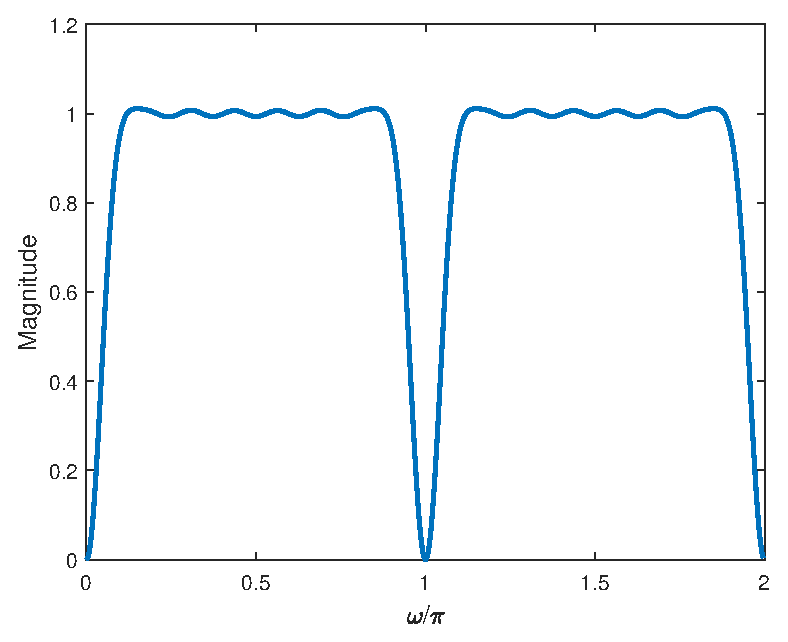
\includegraphics[width=\textwidth]{figs/hilbert_win_mag.eps}
		\caption{Magnitude} 
	\end{subfigure}%
	~ 
	\begin{subfigure}[h!]{0.5\textwidth}
		\includegraphics[width=\textwidth]{figs/hilbert_win_phase.eps}
		\caption{Phase}
	\end{subfigure}
	\caption{(a) magnitude and (b) phase response of Hilbert transformer designed by windowing with Hamming window.}
\end{figure}
\FloatBarrier

See the code for details.

\subsection{(b)}

To design the Hilbert transformer by Parks-McClellan we can simply do
\begin{equation*}
	\texttt{>> hpm = firpm(M, [0.1 0.9], [1 1], `hilbert');}
\end{equation*}
This filter will have constant magnitude between $0.1\pi$ and $0.9\pi$. The parameter \texttt{`hilbert'} guarantees that the filter has odd symmetry.


\FloatBarrier
\begin{figure}[h!]
	\centering
	\begin{subfigure}[h!]{0.5\textwidth}
		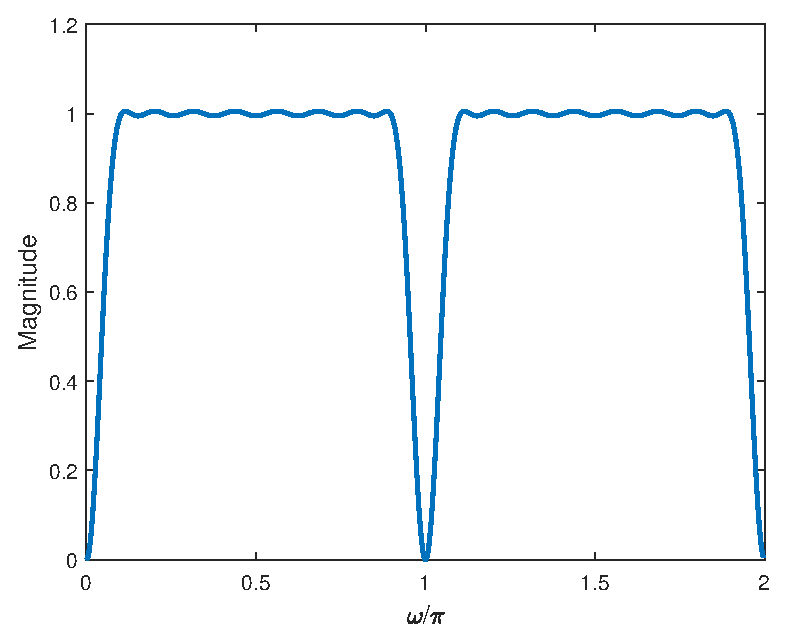
\includegraphics[width=\textwidth]{figs/hilbert_pm_mag.eps}
		\caption{Magnitude} 
	\end{subfigure}%
	~ 
	\begin{subfigure}[h!]{0.5\textwidth}
		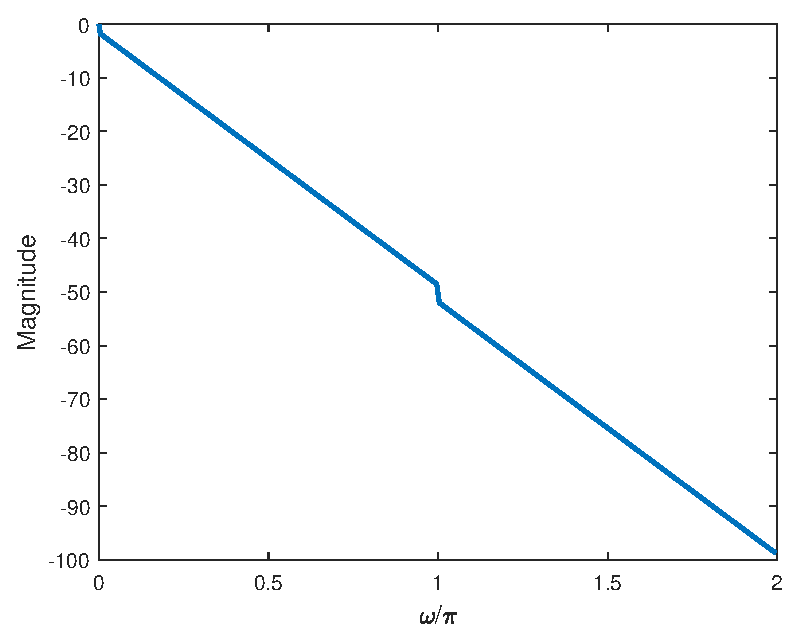
\includegraphics[width=\textwidth]{figs/hilbert_pm_phase.eps}
		\caption{Phase}
	\end{subfigure}
	\caption{(a) magnitude and (b) phase response of Hilbert transformer designed by Parks-McClellan method.}
\end{figure}
\FloatBarrier

See the code for details.

\subsection{(c)}

Similarly to part (c), to design the Hilbert transformer by leasts-squares algorithm we can simply do
\begin{equation*}
\texttt{>> hls = firls(M, [0.1 0.9], [1 1], `hilbert');}
\end{equation*}
This filter will have constant magnitude between $0.1\pi$ and $0.9\pi$. The parameter \texttt{`hilbert'} guarantees that the filter has odd symmetry.

\FloatBarrier
\begin{figure}[h!]
	\centering
	\begin{subfigure}[h!]{0.5\textwidth}
		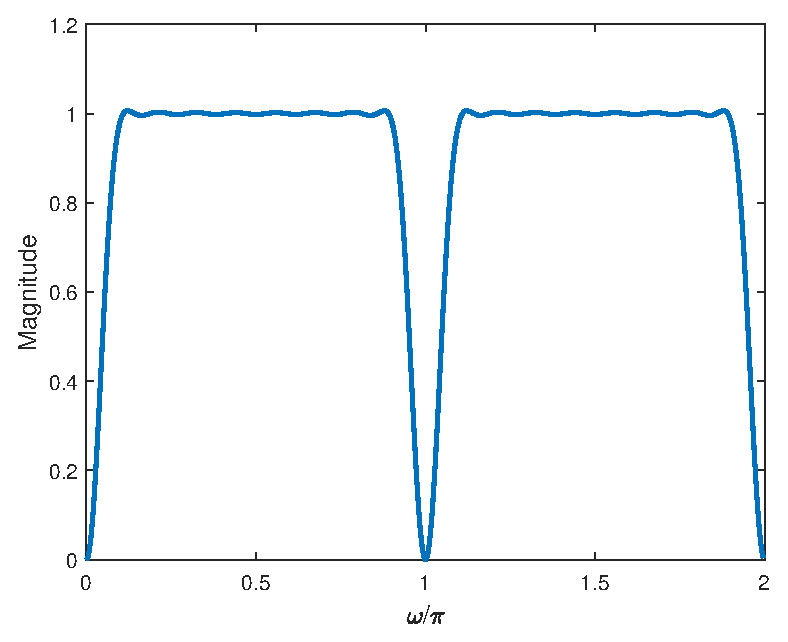
\includegraphics[width=\textwidth]{figs/hilbert_ls_mag.eps}
		\caption{Magnitude} 
	\end{subfigure}%
	~ 
	\begin{subfigure}[h!]{0.5\textwidth}
		\includegraphics[width=\textwidth]{figs/hilbert_ls_phase.eps}
		\caption{Phase}
	\end{subfigure}
	\caption{(a) magnitude and (b) phase response of Hilbert transformer designed by leasts-squares method.}
\end{figure}
\FloatBarrier

See the code for details.

\subsection{Matlab code for Problem 5}
% This file was automatically created from the m-file 
% "m2tex.m" written by USL. 
% The fontencoding in this file is UTF-8. 
%  
% You will need to include the following two packages in 
% your LaTeX-Main-File. 
%  
% \usepackage{color} 
% \usepackage{fancyvrb} 
%  
% It is advised to use the following option for Inputenc 
% \usepackage[utf8]{inputenc} 
%  
  
% definition of matlab colors: 
\definecolor{mblue}{rgb}{0,0,1} 
\definecolor{mgreen}{rgb}{0.13333,0.5451,0.13333} 
\definecolor{mred}{rgb}{0.62745,0.12549,0.94118} 
\definecolor{mgrey}{rgb}{0.5,0.5,0.5} 
\definecolor{mdarkgrey}{rgb}{0.25,0.25,0.25} 
  
\DefineShortVerb[fontfamily=courier,fontseries=m]{\$} 
\DefineShortVerb[fontfamily=courier,fontseries=b]{\#} 
  
\noindent                                                               
 \hspace*{-1.6em}{\scriptsize 1}$  $\color{mgrey}#%% Hilbert transformer#\color{black}$$\\
 \hspace*{-1.6em}{\scriptsize 2}$  clear, $\color{mdarkgrey}$clc, close all$\color{black}$$\\
 \hspace*{-1.6em}{\scriptsize 3}$  $\\
 \hspace*{-1.6em}{\scriptsize 4}$  $\color{mgrey}$% Define parameters$\color{black}$$\\
 \hspace*{-1.6em}{\scriptsize 5}$  L = 31;$\\
 \hspace*{-1.6em}{\scriptsize 6}$  M = L -1;$\\
 \hspace*{-1.6em}{\scriptsize 7}$  $\\
 \hspace*{-1.6em}{\scriptsize 8}$  $\color{mgrey}#%% a) Window method#\color{black}$$\\
 \hspace*{-1.6em}{\scriptsize 9}$  n = -M/2:M/2;$\\
 \hspace*{-2em}{\scriptsize 10}$  hd = 2/pi*((sin(pi*n/2)).^2)./n;$\\
 \hspace*{-2em}{\scriptsize 11}$  hd(n == 0) = 0; $\color{mgrey}$% enforce value at 0$\color{black}$$\\
 \hspace*{-2em}{\scriptsize 12}$  $\\
 \hspace*{-2em}{\scriptsize 13}$  $\color{mgrey}$% window by Hamming window$\color{black}$$\\
 \hspace*{-2em}{\scriptsize 14}$  hwin = hd.*hamming(M+1).';$\\
 \hspace*{-2em}{\scriptsize 15}$  $\\
 \hspace*{-2em}{\scriptsize 16}$  [Hwin, w] = freqz(hwin, 1, $\color{mdarkgrey}$'whole'$\color{black}$);$\\
 \hspace*{-2em}{\scriptsize 17}$  $\\
 \hspace*{-2em}{\scriptsize 18}$  figure, $\color{mdarkgrey}$box on$\color{black}$$\\
 \hspace*{-2em}{\scriptsize 19}$  plot(w/pi, abs(Hwin).^2, $\color{mdarkgrey}$'LineWidth'$\color{black}$, 2)$\\
 \hspace*{-2em}{\scriptsize 20}$  xlabel($\color{mdarkgrey}$'\omega/\pi'$\color{black}$, $\color{mdarkgrey}$'FontSize'$\color{black}$, 12)$\\
 \hspace*{-2em}{\scriptsize 21}$  ylabel($\color{mdarkgrey}$'Magnitude'$\color{black}$, $\color{mdarkgrey}$'FontSize'$\color{black}$, 12)$\\
 \hspace*{-2em}{\scriptsize 22}$  saveas(gca, $\color{mdarkgrey}$'../figs/hilbert_win_mag'$\color{black}$, $\color{mdarkgrey}$'epsc'$\color{black}$)$\\
 \hspace*{-2em}{\scriptsize 23}$  $\\
 \hspace*{-2em}{\scriptsize 24}$  figure, $\color{mdarkgrey}$box on$\color{black}$$\\
 \hspace*{-2em}{\scriptsize 25}$  plot(w/pi, unwrap(angle(Hwin)), $\color{mdarkgrey}$'LineWidth'$\color{black}$, 2)$\\
 \hspace*{-2em}{\scriptsize 26}$  xlabel($\color{mdarkgrey}$'\omega/\pi'$\color{black}$, $\color{mdarkgrey}$'FontSize'$\color{black}$, 12)$\\
 \hspace*{-2em}{\scriptsize 27}$  ylabel($\color{mdarkgrey}$'Magnitude'$\color{black}$, $\color{mdarkgrey}$'FontSize'$\color{black}$, 12)$\\
 \hspace*{-2em}{\scriptsize 28}$  saveas(gca, $\color{mdarkgrey}$'../figs/hilbert_win_phase'$\color{black}$, $\color{mdarkgrey}$'epsc'$\color{black}$)$\\
 \hspace*{-2em}{\scriptsize 29}$  $\\
 \hspace*{-2em}{\scriptsize 30}$  $\color{mgrey}#%% b) Parks-McClellan method#\color{black}$$\\
 \hspace*{-2em}{\scriptsize 31}$  hpm = firpm(M, [0.1 0.9], [1 1], $\color{mdarkgrey}$'hilbert'$\color{black}$);$\\
 \hspace*{-2em}{\scriptsize 32}$  figure, $\color{mdarkgrey}$freqz(hpm, 1)$\color{black}$$\\
 \hspace*{-2em}{\scriptsize 33}$  $\\
 \hspace*{-2em}{\scriptsize 34}$  [Hpm, w] = freqz(hpm, 1, $\color{mdarkgrey}$'whole'$\color{black}$);$\\
 \hspace*{-2em}{\scriptsize 35}$  $\\
 \hspace*{-2em}{\scriptsize 36}$  figure, $\color{mdarkgrey}$box on$\color{black}$$\\
 \hspace*{-2em}{\scriptsize 37}$  plot(w/pi, abs(Hpm).^2, $\color{mdarkgrey}$'LineWidth'$\color{black}$, 2)$\\
 \hspace*{-2em}{\scriptsize 38}$  xlabel($\color{mdarkgrey}$'\omega/\pi'$\color{black}$, $\color{mdarkgrey}$'FontSize'$\color{black}$, 12)$\\
 \hspace*{-2em}{\scriptsize 39}$  ylabel($\color{mdarkgrey}$'Magnitude'$\color{black}$, $\color{mdarkgrey}$'FontSize'$\color{black}$, 12)$\\
 \hspace*{-2em}{\scriptsize 40}$  saveas(gca, $\color{mdarkgrey}$'../figs/hilbert_pm_mag'$\color{black}$, $\color{mdarkgrey}$'epsc'$\color{black}$)$\\
 \hspace*{-2em}{\scriptsize 41}$  $\\
 \hspace*{-2em}{\scriptsize 42}$  figure, $\color{mdarkgrey}$box on$\color{black}$$\\
 \hspace*{-2em}{\scriptsize 43}$  plot(w/pi, unwrap(angle(Hpm)), $\color{mdarkgrey}$'LineWidth'$\color{black}$, 2)$\\
 \hspace*{-2em}{\scriptsize 44}$  xlabel($\color{mdarkgrey}$'\omega/\pi'$\color{black}$, $\color{mdarkgrey}$'FontSize'$\color{black}$, 12)$\\
 \hspace*{-2em}{\scriptsize 45}$  ylabel($\color{mdarkgrey}$'Magnitude'$\color{black}$, $\color{mdarkgrey}$'FontSize'$\color{black}$, 12)$\\
 \hspace*{-2em}{\scriptsize 46}$  saveas(gca, $\color{mdarkgrey}$'../figs/hilbert_pm_phase'$\color{black}$, $\color{mdarkgrey}$'epsc'$\color{black}$)$\\
 \hspace*{-2em}{\scriptsize 47}$  $\\
 \hspace*{-2em}{\scriptsize 48}$  $\color{mgrey}#%% c) Least-squares method#\color{black}$$\\
 \hspace*{-2em}{\scriptsize 49}$  hls = firls(M, [0.1 0.9], [1 1], $\color{mdarkgrey}$'hilbert'$\color{black}$);$\\
 \hspace*{-2em}{\scriptsize 50}$  $\\
 \hspace*{-2em}{\scriptsize 51}$  [Hls, w] = freqz(hls, 1, $\color{mdarkgrey}$'whole'$\color{black}$);$\\
 \hspace*{-2em}{\scriptsize 52}$  $\\
 \hspace*{-2em}{\scriptsize 53}$  figure, $\color{mdarkgrey}$box on$\color{black}$$\\
 \hspace*{-2em}{\scriptsize 54}$  plot(w/pi, abs(Hls).^2, $\color{mdarkgrey}$'LineWidth'$\color{black}$, 2)$\\
 \hspace*{-2em}{\scriptsize 55}$  xlabel($\color{mdarkgrey}$'\omega/\pi'$\color{black}$, $\color{mdarkgrey}$'FontSize'$\color{black}$, 12)$\\
 \hspace*{-2em}{\scriptsize 56}$  ylabel($\color{mdarkgrey}$'Magnitude'$\color{black}$, $\color{mdarkgrey}$'FontSize'$\color{black}$, 12)$\\
 \hspace*{-2em}{\scriptsize 57}$  saveas(gca, $\color{mdarkgrey}$'../figs/hilbert_ls_mag'$\color{black}$, $\color{mdarkgrey}$'epsc'$\color{black}$)$\\
 \hspace*{-2em}{\scriptsize 58}$  $\\
 \hspace*{-2em}{\scriptsize 59}$  figure, $\color{mdarkgrey}$box on$\color{black}$$\\
 \hspace*{-2em}{\scriptsize 60}$  plot(w/pi, unwrap(angle(Hls)), $\color{mdarkgrey}$'LineWidth'$\color{black}$, 2)$\\
 \hspace*{-2em}{\scriptsize 61}$  xlabel($\color{mdarkgrey}$'\omega/\pi'$\color{black}$, $\color{mdarkgrey}$'FontSize'$\color{black}$, 12)$\\
 \hspace*{-2em}{\scriptsize 62}$  ylabel($\color{mdarkgrey}$'Phase (rad)'$\color{black}$, $\color{mdarkgrey}$'FontSize'$\color{black}$, 12)$\\
 \hspace*{-2em}{\scriptsize 63}$  saveas(gca, $\color{mdarkgrey}$'../figs/hilbert_ls_phase'$\color{black}$, $\color{mdarkgrey}$'epsc'$\color{black}$)$\\ 
  
\UndefineShortVerb{\$} 
\UndefineShortVerb{\#}

\newpage
\section{Problem 6}
\subsection{(a)}

For the window method we simply need to make
\begin{equation}
	h_{win}[n] = \begin{cases}
	h[n], n = 0, \ldots, M-1 \\
	0, \text{otherwise}
	\end{cases}
\end{equation}

We can obtain $h[n]$ analytically or by using the \texttt{impz} function from Matlab. 

The magnitude and phase plots of $H(z)$ and the filter designed by windowing $H_{win}(z)$ are shown below. The magnitude is plotted in linear units. Note that the phase is nonlinear.

\FloatBarrier
\begin{figure}[h!]
	\centering
	\begin{subfigure}[h!]{0.5\textwidth}
		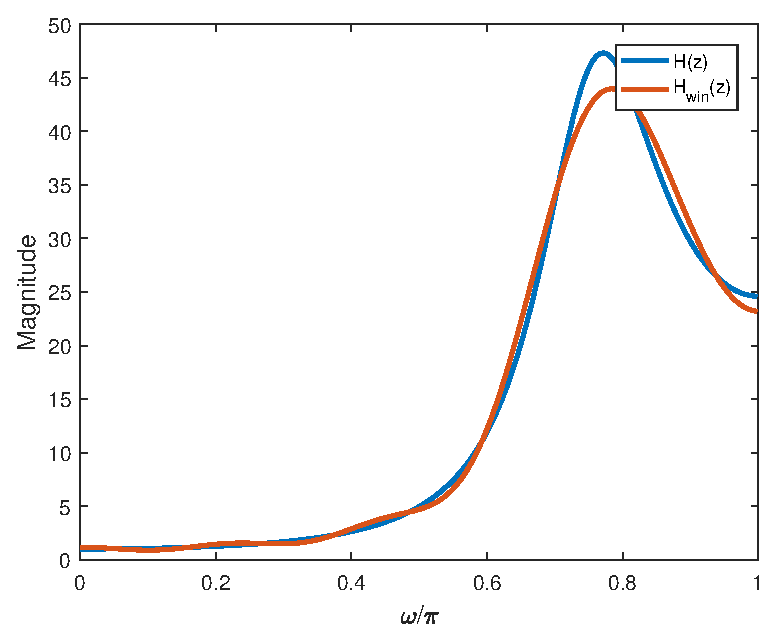
\includegraphics[width=\textwidth]{eq_rect_win_mag.eps}
		\caption{Magnitude}
	\end{subfigure}%
	~ %add desired spacing between images, e. g. ~, \quad, \qquad etc.
	%(or a blank line to force the subfigure onto a new line)
	\begin{subfigure}[h!]{0.5\textwidth}
		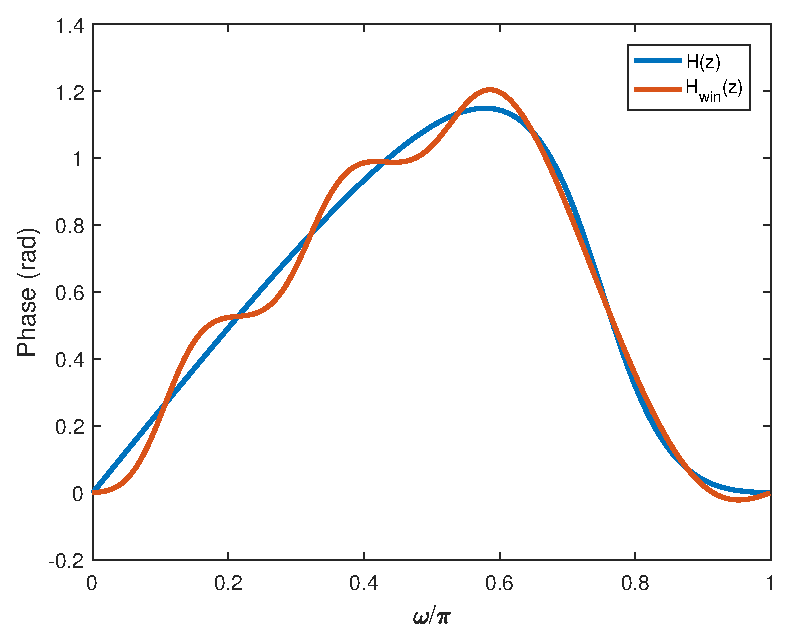
\includegraphics[width=\textwidth]{eq_rect_win_phase.eps}
		\caption{Phase}
	\end{subfigure}
	\caption{(a) Magnitude and (b) phase response of the filter designed by windowing compared to the desired $H(z)$.}
\end{figure}
\FloatBarrier

\subsection{(b)}

\begin{align}
	&\texttt{>> BER = simple\_channel(1) = 0.2442} \tag{without equalization} \\
	&\texttt{>> BER = simple\_channel(hwin) = 0} \tag{with equalization}
\end{align}

Different (but close) values are possible depending on the random number generator seed.

\subsection{(c)}

To design a non-linear phase FIR filter using the least-squares algorithm, we need to define the matrix $Q$ as done in lecture notes 9, slide 49. The code to generate this matrix was available on Canvas/Files/Matlab: \texttt{predicing\_bandlimited\_signals.m}.

Once the matrix $Q$, we can use least-squares as usual:
\begin{equation}
h = Q^\dagger d
\end{equation}
since the weight matrix $W$ is equal to the identity.

This results in the following magnitude and phase responses:
\FloatBarrier
\begin{figure}[h!]
	\centering
	\begin{subfigure}[h!]{0.5\textwidth}
		\includegraphics[width=\textwidth]{eq_ls_mag.eps}
		\caption{Magnitude}
	\end{subfigure}%
	~ %add desired spacing between images, e. g. ~, \quad, \qquad etc.
	%(or a blank line to force the subfigure onto a new line)
	\begin{subfigure}[h!]{0.5\textwidth}
		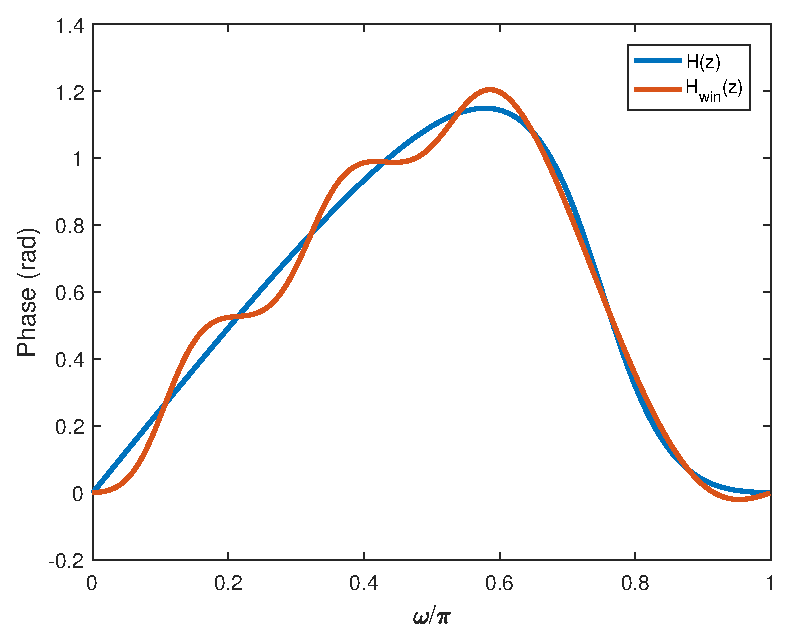
\includegraphics[width=\textwidth]{eq_ls_phase.eps}
		\caption{Phase}
	\end{subfigure}
	\caption{(a) Magnitude and (b) phase response of the filter designed by leasts-squares compared to the desired $H(z)$.}
\end{figure}
\FloatBarrier

As expected, this is identical to the result obtained by windoing. This only happens because in this case the weight function was one everywhere i.e., the matrix $Q$ was the identity.

\subsection{(d)}

The noise is filtered by $H_{win}(z) = H_{ls}(z)$. Therefore, the noise PSD is shaped by
\begin{align}
	\Phi_{ff}(e^{j\omega}) = \sigma^2|H_{win}(e^{j\omega})|^2
\end{align}

Hence, the total power after filtering is
\begin{align}
	\sigma_f^2 &= \frac{\sigma^2}{2\pi}\int_{-\pi}^{\pi}|H_{win}(e^{j\omega})|^2d\omega \\
	&= \sum_{m=0}^{M} |h_{win}[m]|^2 \\
	&= 0.0144
\end{align}

This value is 14 times larger than $\sigma^2$.

\subsection{Matlab code for problem 6}
% This file was automatically created from the m-file 
% "m2tex.m" written by USL. 
% The fontencoding in this file is UTF-8. 
%  
% You will need to include the following two packages in 
% your LaTeX-Main-File. 
%  
% \usepackage{color} 
% \usepackage{fancyvrb} 
%  
% It is advised to use the following option for Inputenc 
% \usepackage[utf8]{inputenc} 
%  
  
% definition of matlab colors: 
\definecolor{mblue}{rgb}{0,0,1} 
\definecolor{mgreen}{rgb}{0.13333,0.5451,0.13333} 
\definecolor{mred}{rgb}{0.62745,0.12549,0.94118} 
\definecolor{mgrey}{rgb}{0.5,0.5,0.5} 
\definecolor{mdarkgrey}{rgb}{0.25,0.25,0.25} 
  
\DefineShortVerb[fontfamily=courier,fontseries=m]{\$} 
\DefineShortVerb[fontfamily=courier,fontseries=b]{\#} 
  
\noindent                                                                                  
 \hspace*{-1.6em}{\scriptsize 1}$  $\color{mgrey}#%% Linear equalization#\color{black}$$\\
 \hspace*{-1.6em}{\scriptsize 2}$  clear, $\color{mdarkgrey}$clc, close all$\color{black}$$\\
 \hspace*{-1.6em}{\scriptsize 3}$  $\\
 \hspace*{-1.6em}{\scriptsize 4}$  M = 8; $\color{mgrey}$% Filter order$\color{black}$$\\
 \hspace*{-1.6em}{\scriptsize 5}$  $\\
 \hspace*{-1.6em}{\scriptsize 6}$  $\color{mgrey}$% Filter coefficients$\color{black}$$\\
 \hspace*{-1.6em}{\scriptsize 7}$  c = [0.4032    0.3992    0.1976];$\\
 \hspace*{-1.6em}{\scriptsize 8}$  $\\
 \hspace*{-1.6em}{\scriptsize 9}$  $\color{mgrey}$% Impulse response of 1/C(z)$\color{black}$$\\
 \hspace*{-2em}{\scriptsize 10}$  hc = impz(1, c);$\\
 \hspace*{-2em}{\scriptsize 11}$  $\\
 \hspace*{-2em}{\scriptsize 12}$  $\color{mgrey}#%% a) Window method with rectangular window#\color{black}$$\\
 \hspace*{-2em}{\scriptsize 13}$  hwin = hc(1:M+1);$\\
 \hspace*{-2em}{\scriptsize 14}$  $\\
 \hspace*{-2em}{\scriptsize 15}$  BER = simple_channel(hwin)$\\
 \hspace*{-2em}{\scriptsize 16}$  $\\
 \hspace*{-2em}{\scriptsize 17}$  $\color{mgrey}$% Plot results$\color{black}$$\\
 \hspace*{-2em}{\scriptsize 18}$  [H, $\color{mdarkgrey}$w] = freqz(1, c);$\color{black}$$\\
 \hspace*{-2em}{\scriptsize 19}$  Hwin = freqz(hwin, 1, w);$\\
 \hspace*{-2em}{\scriptsize 20}$  $\\
 \hspace*{-2em}{\scriptsize 21}$  figure, $\color{mdarkgrey}$hold on, box on$\color{black}$$\\
 \hspace*{-2em}{\scriptsize 22}$  plot(w/pi, abs(H).^2, $\color{mdarkgrey}$'LineWidth'$\color{black}$, 2, $\color{mdarkgrey}$'displayname'$\color{black}$, $\color{mdarkgrey}$'H(z)'$\color{black}$)$\\
 \hspace*{-2em}{\scriptsize 23}$  plot(w/pi, abs(Hwin).^2, $\color{mdarkgrey}$'LineWidth'$\color{black}$, 2, $\color{mdarkgrey}$'displayname'$\color{black}$, $\color{mdarkgrey}$'H_{win}(z)'$\color{black}$)$\\
 \hspace*{-2em}{\scriptsize 24}$  xlabel($\color{mdarkgrey}$'\omega/\pi'$\color{black}$, $\color{mdarkgrey}$'FontSize'$\color{black}$, 12)$\\
 \hspace*{-2em}{\scriptsize 25}$  ylabel($\color{mdarkgrey}$'Magnitude'$\color{black}$, $\color{mdarkgrey}$'FontSize'$\color{black}$, 12)$\\
 \hspace*{-2em}{\scriptsize 26}$  legend($\color{mdarkgrey}$'-dynamiclegend'$\color{black}$)$\\
 \hspace*{-2em}{\scriptsize 27}$  saveas(gca, $\color{mdarkgrey}$'../figs/eq_rect_win_mag'$\color{black}$, $\color{mdarkgrey}$'epsc'$\color{black}$)$\\
 \hspace*{-2em}{\scriptsize 28}$  $\\
 \hspace*{-2em}{\scriptsize 29}$  figure, $\color{mdarkgrey}$hold on, box on$\color{black}$$\\
 \hspace*{-2em}{\scriptsize 30}$  plot(w/pi, unwrap(angle(H)), $\color{mdarkgrey}$'LineWidth'$\color{black}$, 2, $\color{mdarkgrey}$'displayname'$\color{black}$, $\color{mdarkgrey}$'H(z)'$\color{black}$)$\\
 \hspace*{-2em}{\scriptsize 31}$  plot(w/pi, unwrap(angle(Hwin)), $\color{mdarkgrey}$'LineWidth'$\color{black}$, 2, $\color{mdarkgrey}$'displayname'$\color{black}$, $\color{mdarkgrey}$'H_{win}(z)'$\color{black}$)$\\
 \hspace*{-2em}{\scriptsize 32}$  xlabel($\color{mdarkgrey}$'\omega/\pi'$\color{black}$, $\color{mdarkgrey}$'FontSize'$\color{black}$, 12)$\\
 \hspace*{-2em}{\scriptsize 33}$  ylabel($\color{mdarkgrey}$'Phase (rad)'$\color{black}$, $\color{mdarkgrey}$'FontSize'$\color{black}$, 12)$\\
 \hspace*{-2em}{\scriptsize 34}$  legend($\color{mdarkgrey}$'-dynamiclegend'$\color{black}$)$\\
 \hspace*{-2em}{\scriptsize 35}$  saveas(gca, $\color{mdarkgrey}$'../figs/eq_rect_win_phase'$\color{black}$, $\color{mdarkgrey}$'epsc'$\color{black}$)$\\
 \hspace*{-2em}{\scriptsize 36}$  $\\
 \hspace*{-2em}{\scriptsize 37}$  $\color{mgrey}#%% c) Least-squares method#\color{black}$$\\
 \hspace*{-2em}{\scriptsize 38}$  $\color{mgrey}$% Calculate matrix Q$\color{black}$$\\
 \hspace*{-2em}{\scriptsize 39}$  $\color{mgrey}$% This assumes even symmetry$\color{black}$$\\
 \hspace*{-2em}{\scriptsize 40}$  N = 100;$\\
 \hspace*{-2em}{\scriptsize 41}$  w = linspace(-pi, pi).';$\\
 \hspace*{-2em}{\scriptsize 42}$  d = freqz(1, c, w);$\\
 \hspace*{-2em}{\scriptsize 43}$  $\\
 \hspace*{-2em}{\scriptsize 44}$  Q = zeros(N, M+1); $\color{mgrey}$% initialized$\color{black}$$\\
 \hspace*{-2em}{\scriptsize 45}$  n = 0:M; $\color{mgrey}$% time vector$\color{black}$$\\
 \hspace*{-2em}{\scriptsize 46}$  $#for#$ i = 1:N $\color{mgrey}$% for every frequency wi$\color{black}$$\\
 \hspace*{-2em}{\scriptsize 47}$      Q(i, $\color{mdarkgrey}$:) = exp(-1j*w(i)*n);$\color{black}$$\\
 \hspace*{-2em}{\scriptsize 48}$  $#end#$$\\
 \hspace*{-2em}{\scriptsize 49}$  $\\
 \hspace*{-2em}{\scriptsize 50}$  $\color{mgrey}$% Least-squares filter$\color{black}$$\\
 \hspace*{-2em}{\scriptsize 51}$  hls = pinv(Q)*d;$\\
 \hspace*{-2em}{\scriptsize 52}$  $\\
 \hspace*{-2em}{\scriptsize 53}$  BER = simple_channel(hls)$\\
 \hspace*{-2em}{\scriptsize 54}$  $\\
 \hspace*{-2em}{\scriptsize 55}$  $\color{mgrey}$% Plot results$\color{black}$$\\
 \hspace*{-2em}{\scriptsize 56}$  [H, $\color{mdarkgrey}$w] = freqz(1, c);$\color{black}$$\\
 \hspace*{-2em}{\scriptsize 57}$  Hls = freqz(hls, 1, w);$\\
 \hspace*{-2em}{\scriptsize 58}$  $\\
 \hspace*{-2em}{\scriptsize 59}$  figure, $\color{mdarkgrey}$hold on, box on$\color{black}$$\\
 \hspace*{-2em}{\scriptsize 60}$  plot(w/pi, abs(H).^2, $\color{mdarkgrey}$'LineWidth'$\color{black}$, 2, $\color{mdarkgrey}$'displayname'$\color{black}$, $\color{mdarkgrey}$'H(z)'$\color{black}$)$\\
 \hspace*{-2em}{\scriptsize 61}$  plot(w/pi, abs(Hls).^2, $\color{mdarkgrey}$'LineWidth'$\color{black}$, 2, $\color{mdarkgrey}$'displayname'$\color{black}$, $\color{mdarkgrey}$'H_{win}(z)'$\color{black}$)$\\
 \hspace*{-2em}{\scriptsize 62}$  xlabel($\color{mdarkgrey}$'\omega/\pi'$\color{black}$, $\color{mdarkgrey}$'FontSize'$\color{black}$, 12)$\\
 \hspace*{-2em}{\scriptsize 63}$  ylabel($\color{mdarkgrey}$'Magnitude'$\color{black}$, $\color{mdarkgrey}$'FontSize'$\color{black}$, 12)$\\
 \hspace*{-2em}{\scriptsize 64}$  legend($\color{mdarkgrey}$'-dynamiclegend'$\color{black}$)$\\
 \hspace*{-2em}{\scriptsize 65}$  saveas(gca, $\color{mdarkgrey}$'../figs/eq_ls_mag'$\color{black}$, $\color{mdarkgrey}$'epsc'$\color{black}$)$\\
 \hspace*{-2em}{\scriptsize 66}$  $\\
 \hspace*{-2em}{\scriptsize 67}$  figure, $\color{mdarkgrey}$hold on, box on$\color{black}$$\\
 \hspace*{-2em}{\scriptsize 68}$  plot(w/pi, unwrap(angle(H)), $\color{mdarkgrey}$'LineWidth'$\color{black}$, 2, $\color{mdarkgrey}$'displayname'$\color{black}$, $\color{mdarkgrey}$'H(z)'$\color{black}$)$\\
 \hspace*{-2em}{\scriptsize 69}$  plot(w/pi, unwrap(angle(Hls)), $\color{mdarkgrey}$'LineWidth'$\color{black}$, 2, $\color{mdarkgrey}$'displayname'$\color{black}$, $\color{mdarkgrey}$'H_{win}(z)'$\color{black}$)$\\
 \hspace*{-2em}{\scriptsize 70}$  xlabel($\color{mdarkgrey}$'\omega/\pi'$\color{black}$, $\color{mdarkgrey}$'FontSize'$\color{black}$, 12)$\\
 \hspace*{-2em}{\scriptsize 71}$  ylabel($\color{mdarkgrey}$'Phase (rad)'$\color{black}$, $\color{mdarkgrey}$'FontSize'$\color{black}$, 12)$\\
 \hspace*{-2em}{\scriptsize 72}$  legend($\color{mdarkgrey}$'-dynamiclegend'$\color{black}$)$\\
 \hspace*{-2em}{\scriptsize 73}$  saveas(gca, $\color{mdarkgrey}$'../figs/eq_ls_phase'$\color{black}$, $\color{mdarkgrey}$'epsc'$\color{black}$)$\\
 \hspace*{-2em}{\scriptsize 74}$  $\\
 \hspace*{-2em}{\scriptsize 75}$  $\color{mgrey}$% d)$\color{black}$$\\
 \hspace*{-2em}{\scriptsize 76}$  sigma2 = 0.001;$\\
 \hspace*{-2em}{\scriptsize 77}$  P = sigma2/(pi)*trapz(w, abs(Hls).^2) $\\
 \hspace*{-2em}{\scriptsize 78}$  $\color{mgrey}$% Note division by pi instead of 2pi since w is defined in the interval (0,$\color{black}$$\\
 \hspace*{-2em}{\scriptsize 79}$  $\color{mgrey}$% pi)$\color{black}$$\\
 \hspace*{-2em}{\scriptsize 80}$  $\\
 \hspace*{-2em}{\scriptsize 81}$  $\color{mgrey}$% Another way to calculate P$\color{black}$$\\
 \hspace*{-2em}{\scriptsize 82}$  P = sigma2*sum(abs(hls).^2) $\color{mgrey}$% from Parseval's identity$\color{black}$$\\ 
  
\UndefineShortVerb{\$} 
\UndefineShortVerb{\#}

\end{document}